\documentclass[12pt,a4paper]{article}
\usepackage[utf8]{inputenc}
\usepackage[T1]{fontenc}
\usepackage{mathptmx}
\usepackage{amsmath}
\usepackage{amsfonts}
\usepackage{amssymb}
\usepackage{graphicx}
\usepackage{hyperref}
\usepackage{geometry}
\usepackage{float}
\geometry{a4paper, margin=1in}

\title{\vspace{2cm}\textbf{CPV301 --- Computer Vision}\\
\vspace{0.5cm}\Large{Assignment (Group Project):}\\
\Large{Satellite Image Analysis of Da Nang with Sentinel-2}}
\author{Group: 3}
\date{\today}

\begin{document}

\maketitle
\thispagestyle{empty}
\newpage

\tableofcontents
\newpage

\section{Phase 0: Setup \& Data Collection}

\subsection{Area of Interest (AOI) and Dataset}
For this project, we have collected Sentinel-2 Level-2A satellite imagery over our chosen Area of Interest (AOI) in Da Nang. To track temporal changes, we selected two distinct observation dates: April 11, 2024, and April 11, 2026. The imagery was deliberately exported in two overlapping pieces (an upper half and a lower half) for each date to simulate real-world constraints where large geographic extents exceed single-export pixel limits. This dataset will serve as the foundation for our feature alignment, image stitching, and change detection pipeline.

The collected dataset contains 20 GeoTIFF files in total: four true-color visual previews and sixteen single-band raster files. For each date and crop, we exported the visible Blue, Green, and Red bands (B02, B03, B04), the Near-Infrared band (B08), and one true-color composite. Only the four true-color composites are shown below as a compact dataset overview; the individual spectral bands are retained as processing inputs for NDVI computation, segmentation, alignment, and change tracking.

\begin{figure}[H]
    \centering
    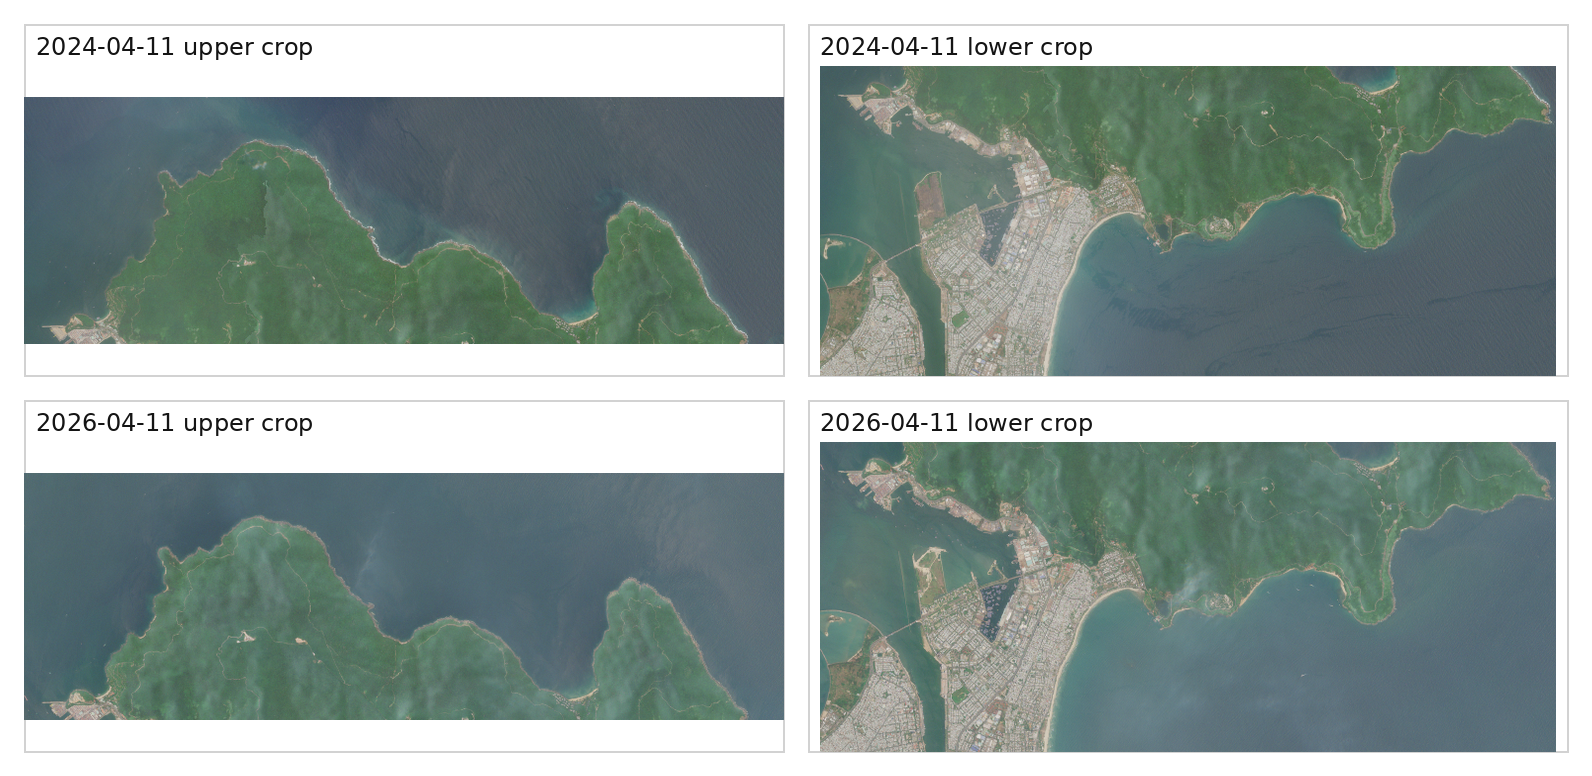
\includegraphics[width=0.98\textwidth]{../output/phase0_dataset_overview.png}
    \caption{Representative true-color Sentinel-2 images collected for the AOI. The dataset covers two dates and two overlapping crops per date.}
    \label{fig:phase0_dataset_overview}
\end{figure}

\begin{table}[H]
    \centering
    \small
    \caption{Collected Sentinel-2 dataset summary.}
    \label{tab:phase0_dataset_summary}
    \begin{tabular}{l l c l}
        \hline
        Date & Crop & Files & True-color size \\
        \hline
        2024-04-11 & Upper & 5 & $774 \times 252$ px \\
        2024-04-11 & Lower & 5 & $743 \times 313$ px \\
        2026-04-11 & Upper & 5 & $774 \times 252$ px \\
        2026-04-11 & Lower & 5 & $743 \times 313$ px \\
        \hline
    \end{tabular}
\end{table}

\subsection{Sentinel-2 Multispectral Image Formation vs. Standard RGB Cameras}
Multispectral satellite imaging, such as that performed by the Copernicus Sentinel-2 mission, differs fundamentally from everyday RGB camera photography across several dimensions:

\begin{itemize}
    \item \textbf{Number and Type of Bands:} While a standard RGB camera captures only three broad bands of visible light (Red, Green, Blue) to mimic human vision, Sentinel-2 captures 13 distinct spectral bands. These span from visible light to Near-Infrared (NIR) and Shortwave-Infrared (SWIR), allowing for advanced environmental analysis beyond what the human eye can perceive.
    \item \textbf{Spatial Resolution:} Everyday cameras take high-resolution images where a pixel might represent millimeters or centimeters. Sentinel-2 is a remote sensing platform operating from orbit; thus, its spatial resolution ranges from $10\text{ m/pixel}$ (for visible and NIR bands) to $60\text{ m/pixel}$ (for atmospheric observation bands).
    \item \textbf{Revisit Time:} A handheld camera captures an instantaneous moment whenever the user desires. In contrast, the Sentinel-2 constellation (comprising 2A and 2B satellites) follows a fixed sun-synchronous orbit, resulting in a revisit time of approximately 5 days at the equator to capture the exact same geographic location under similar lighting conditions.
    \item \textbf{Image Formation (Lens Focal Length):} Traditional cameras utilize a central perspective lens system with a defined focal length to focus an entire 2D scene onto a sensor array simultaneously. Sentinel-2, however, employs a "push-broom" scanner. It does not have a single "lens focal length" in the traditional sense; instead, a linear array of sensors continuously records single lines of pixels perpendicular to the satellite's flight path. The 2D image is mathematically constructed as the satellite moves forward.
\end{itemize}

\subsection{Spectral Bands Utilized}
For the scope of our analysis, we rely on four primary bands provided by the Sentinel-2 Level-2A product:
\begin{itemize}
    \item \textbf{Band 2 (Blue), Band 3 (Green), Band 4 (Red):} These bands measure reflectance in the visible light spectrum. We utilize them to construct True-Color composites, enabling human-interpretable visualization of urban structures, coastlines, and water bodies.
    \item \textbf{Band 8 (Near-Infrared - NIR):} This band measures reflectance in the near-infrared spectrum, which is invisible to the human eye. It is highly sensitive to the cellular structure of healthy leaves, which strongly reflect NIR radiation. We utilize this band in conjunction with the Red band to compute the Normalized Difference Vegetation Index (NDVI), a crucial metric for distinguishing vegetation from built-up urban areas.
\end{itemize}

\section{Phase 1: Image Processing}

\subsection{Objective and Input Data}
The objective of Phase 1 is to apply point operations and basic image enhancement techniques to the Sentinel-2 image pair. Since the AOI was exported in two pieces, the upper crop and lower crop are processed independently in this phase. Image stitching is intentionally left for Phase 3.

For each date, April 11, 2024 and April 11, 2026, we use Band 4 (Red) and Band 8 (Near-Infrared) to compute NDVI. Before computing NDVI, the implementation checks that the Red and NIR bands have matching image dimensions for each crop.

\subsection{NDVI Computation}
The Normalized Difference Vegetation Index (NDVI) is computed as a band-by-band point operation:

\begin{equation}
    NDVI = \frac{NIR - Red}{NIR + Red}
\end{equation}

High NDVI values usually indicate healthy vegetation because vegetation reflects strongly in the NIR band and absorbs more red light. Low or negative NDVI values usually correspond to water, built-up areas, bare soil, shadows, or other non-vegetated surfaces.

\begin{figure}[H]
    \centering
    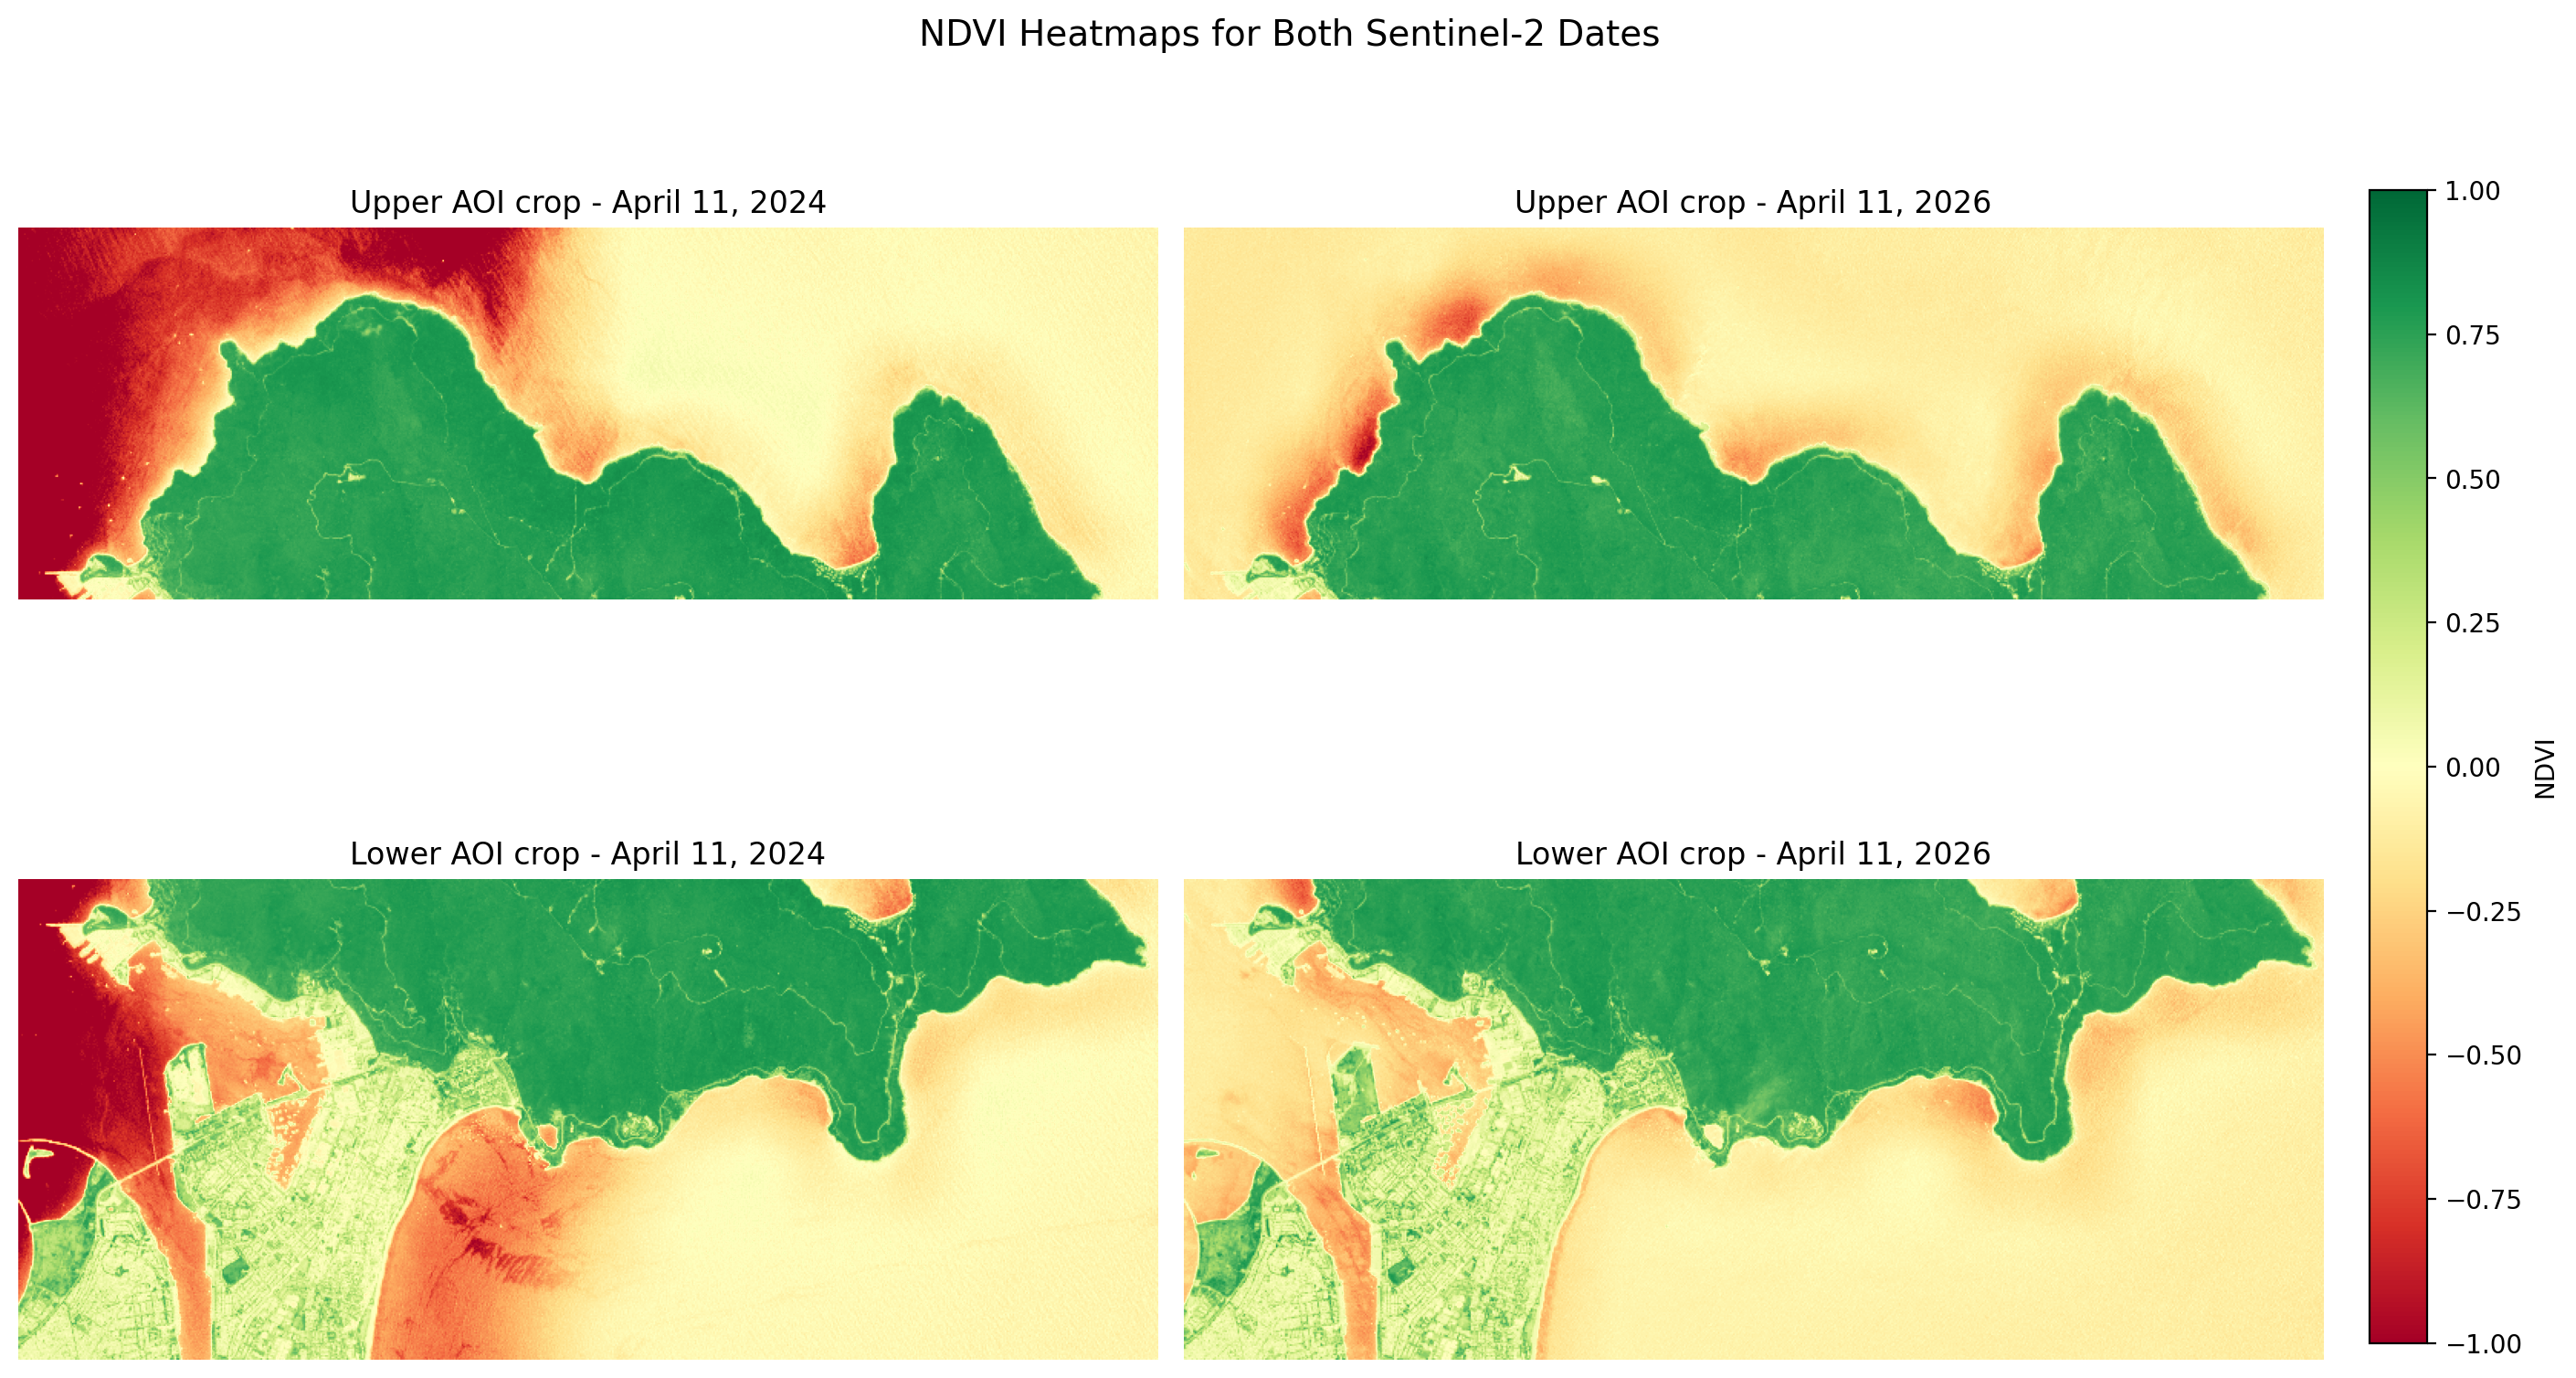
\includegraphics[width=0.98\textwidth]{../output/phase1_ndvi_heatmaps.png}
    \caption{NDVI heatmaps for the upper and lower AOI crops in 2024 and 2026. Green regions indicate higher NDVI values, while red/yellow regions indicate lower NDVI values.}
    \label{fig:phase1_ndvi_heatmaps}
\end{figure}

\subsection{NDVI Quantitative Comparison}
The mean NDVI increased in both AOI crops from 2024 to 2026. The upper crop increased from 0.0711 to 0.1769, while the lower crop increased from 0.1114 to 0.1887. This suggests a net increase in vegetation-like spectral response across both exported pieces of the AOI. The interpretation should still be treated carefully because NDVI can also be affected by cloud shadows, atmospheric differences, water turbidity, and slight geometric offsets.

\begin{table}[H]
    \centering
    \caption{NDVI summary statistics for both AOI crops and both dates.}
    \label{tab:phase1_ndvi_stats}
    \begin{tabular}{l l r r r r}
        \hline
        Crop & Date & Min & Max & Mean & Std. Dev. \\
        \hline
        Upper & 2024 & -1.0000 & 0.8590 & 0.0711 & 0.6043 \\
        Upper & 2026 & -1.0000 & 0.8496 & 0.1769 & 0.4408 \\
        Lower & 2024 & -1.0000 & 0.8526 & 0.1114 & 0.5089 \\
        Lower & 2026 & -0.7572 & 0.8445 & 0.1887 & 0.3933 \\
        \hline
    \end{tabular}
\end{table}

\begin{figure}[H]
    \centering
    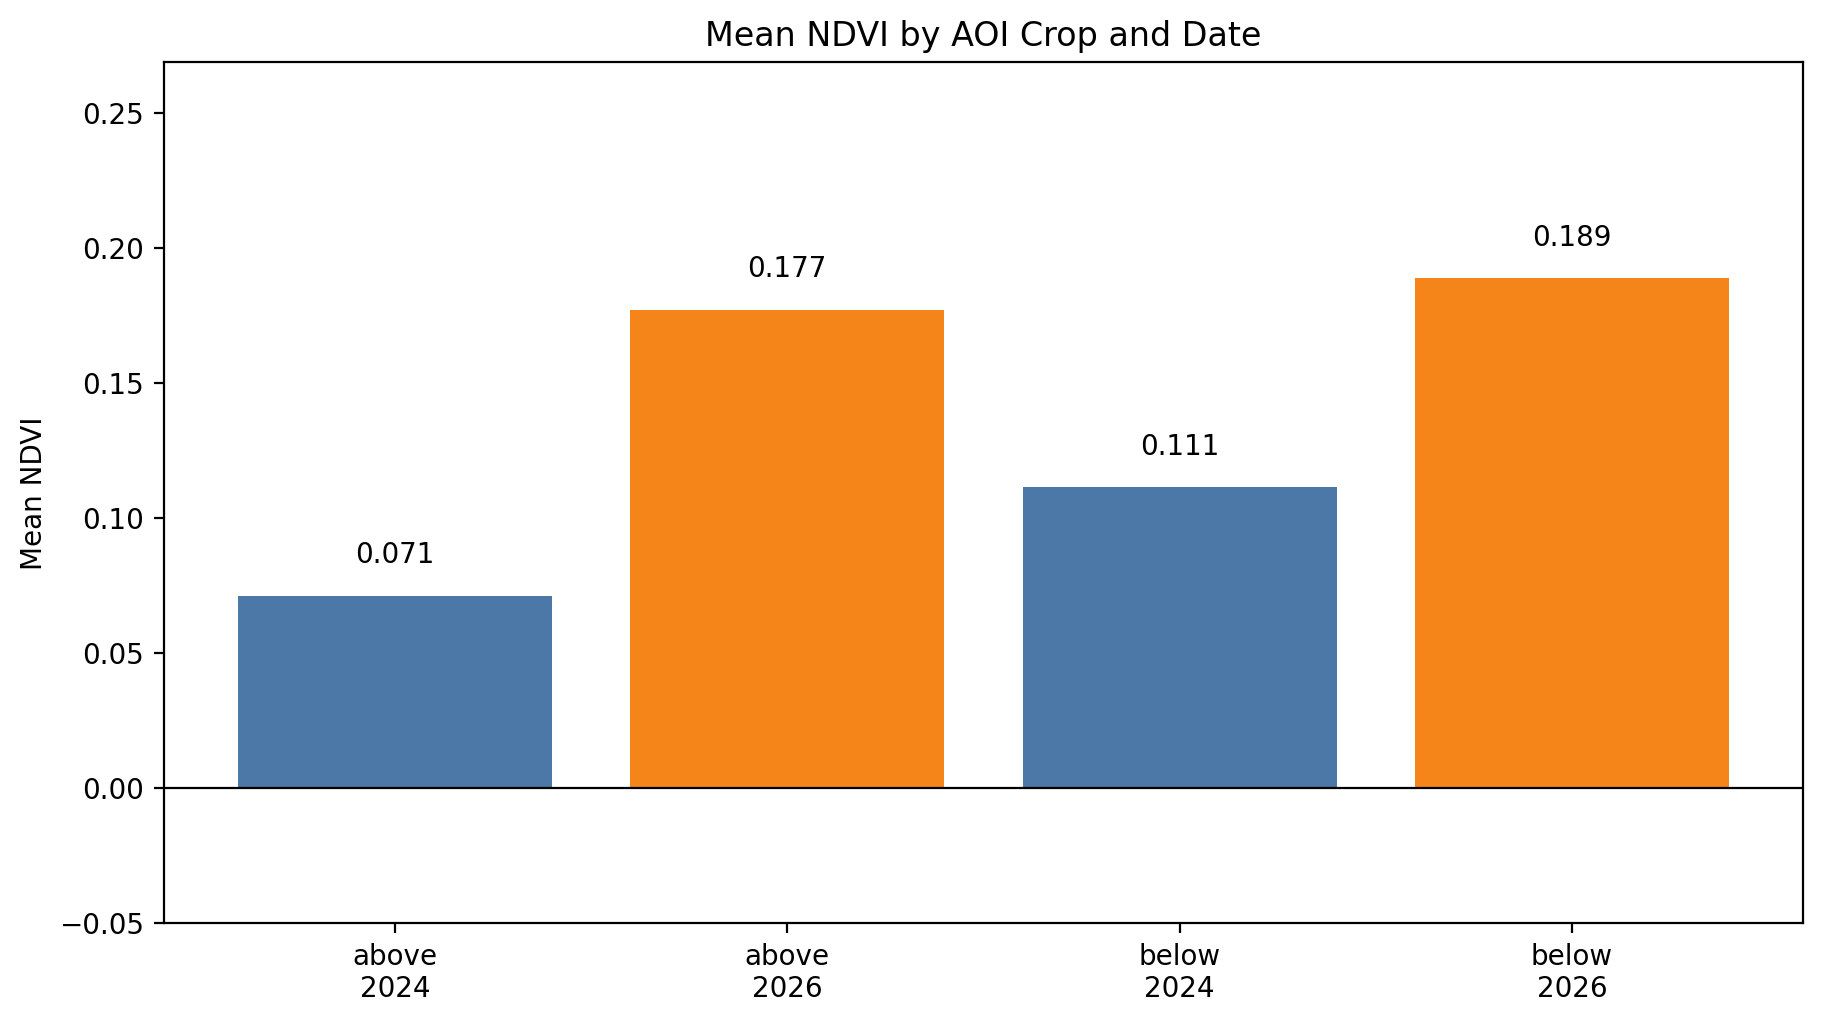
\includegraphics[width=0.85\textwidth]{../output/phase1_ndvi_mean_comparison.png}
    \caption{Mean NDVI comparison between 2024 and 2026 for the upper and lower AOI crops.}
    \label{fig:phase1_ndvi_mean_comparison}
\end{figure}

\begin{figure}[H]
    \centering
    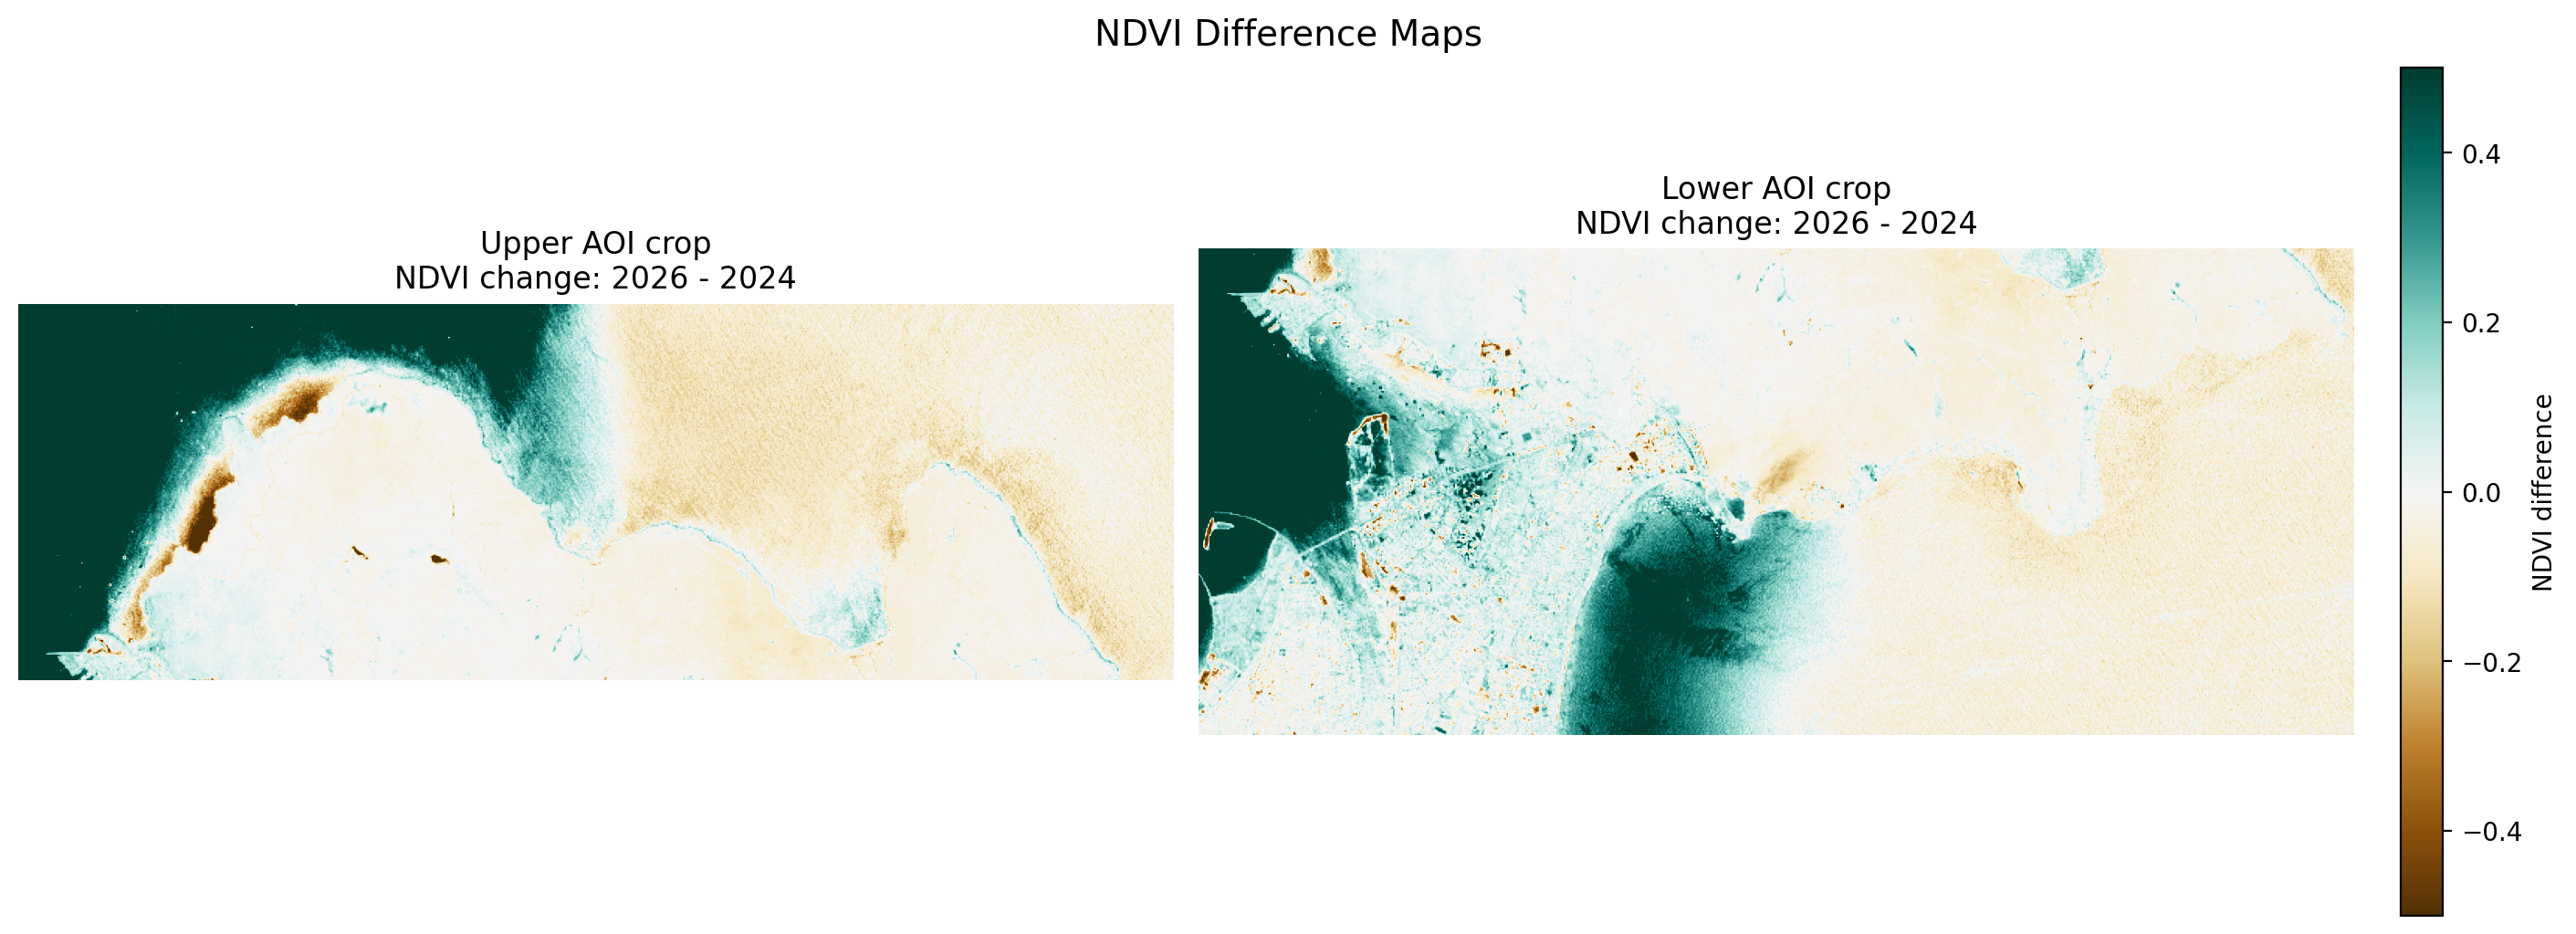
\includegraphics[width=0.98\textwidth]{../output/phase1_ndvi_difference.png}
    \caption{NDVI difference maps computed as 2026 NDVI minus 2024 NDVI. Positive values indicate areas where NDVI increased, while negative values indicate areas where NDVI decreased.}
    \label{fig:phase1_ndvi_difference}
\end{figure}

\subsection{Denoising and Contrast Enhancement}
For image smoothing, we apply a Gaussian blur with a $5 \times 5$ kernel to the true-color image. This filter reduces high-frequency sensor noise and small texture variations, but it can slightly soften thin boundaries such as roads, coastlines, and small construction edges.

For contrast enhancement, we apply histogram equalization to the Value channel in HSV color space. Applying equalization only to the brightness channel improves visual interpretability while reducing color distortion compared with equalizing each RGB channel independently. The trade-off is that weak noise or compression artifacts may become more visible in low-texture areas.

\begin{figure}[H]
    \centering
    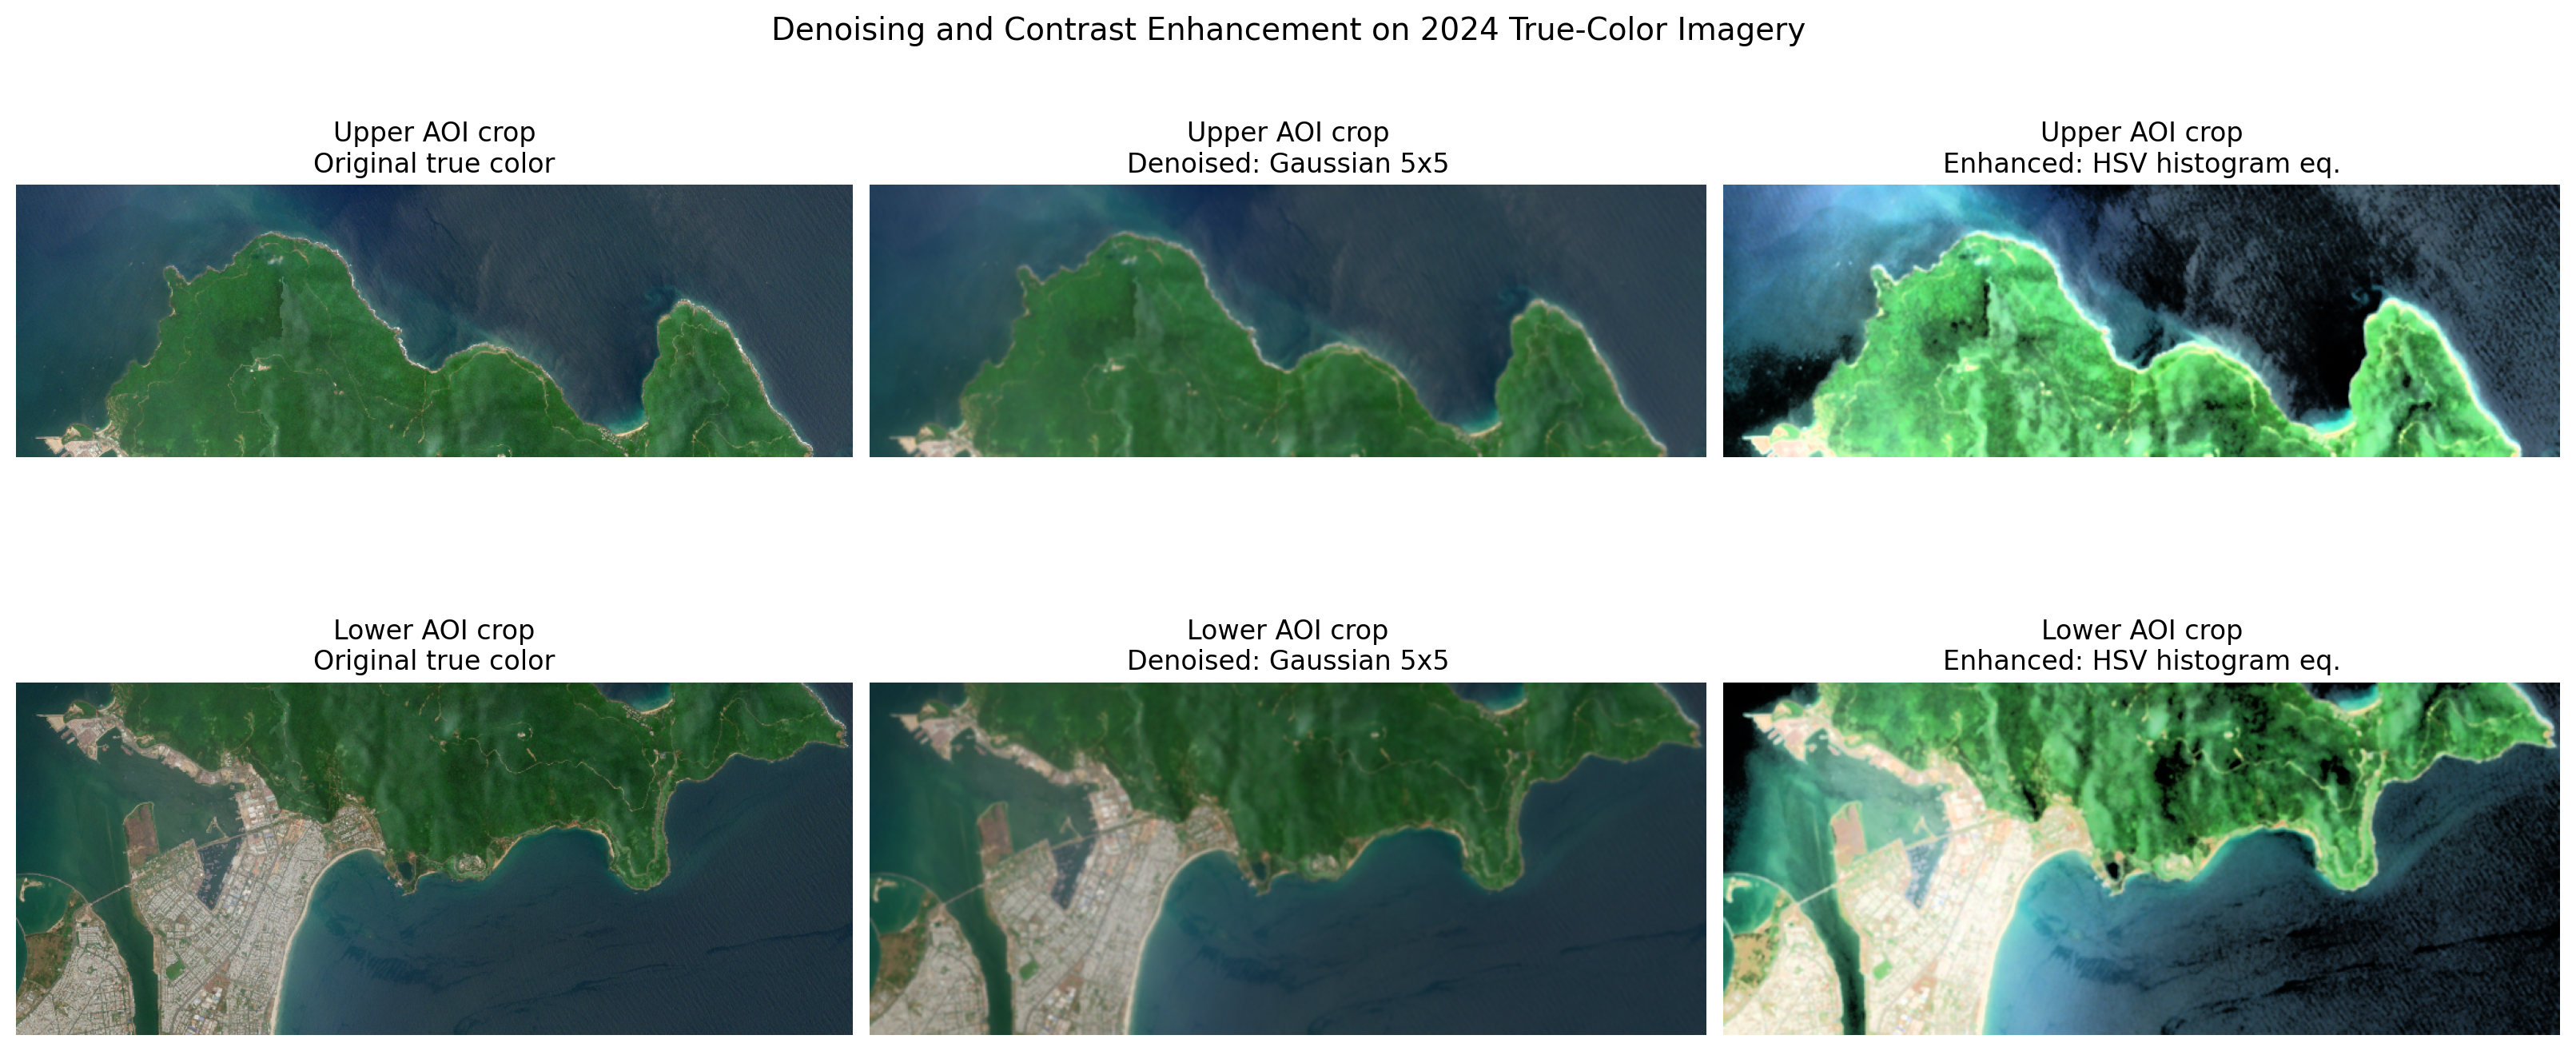
\includegraphics[width=1.0\textwidth]{../output/phase1_filter_contrast_comparison.png}
    \caption{Before/after comparison for the 2024 true-color imagery. Each AOI crop is shown as original true color, Gaussian-denoised output, and HSV histogram-equalized output.}
    \label{fig:phase1_filter_contrast_comparison}
\end{figure}



\section{Phase 2: Segmentation \& Features}
In this phase, we apply advanced feature detection and image segmentation algorithms to delineate structural boundaries and classify land-cover regions across the 2024 imagery.

\subsection{Feature and Edge Detection}
To identify distinct physical boundaries---such as coastlines, road networks, and building footprints---we employed two computer vision techniques:
\begin{itemize}
    \item \textbf{Canny Edge Detection:} Applied to a Gaussian-smoothed grayscale image. Canny effectively extracted high-contrast continuous edges, particularly highlighting major road infrastructures and the sharp coastline boundary between the land and the ocean.
    \item \textbf{ORB (Oriented FAST and Rotated BRIEF):} Used for keypoint detection. ORB detected highly textured regions, heavily clustering around dense urban fabrics and complex port structures, while leaving smooth regions like open water largely empty.
\end{itemize}

\begin{figure}[H]
    \centering
    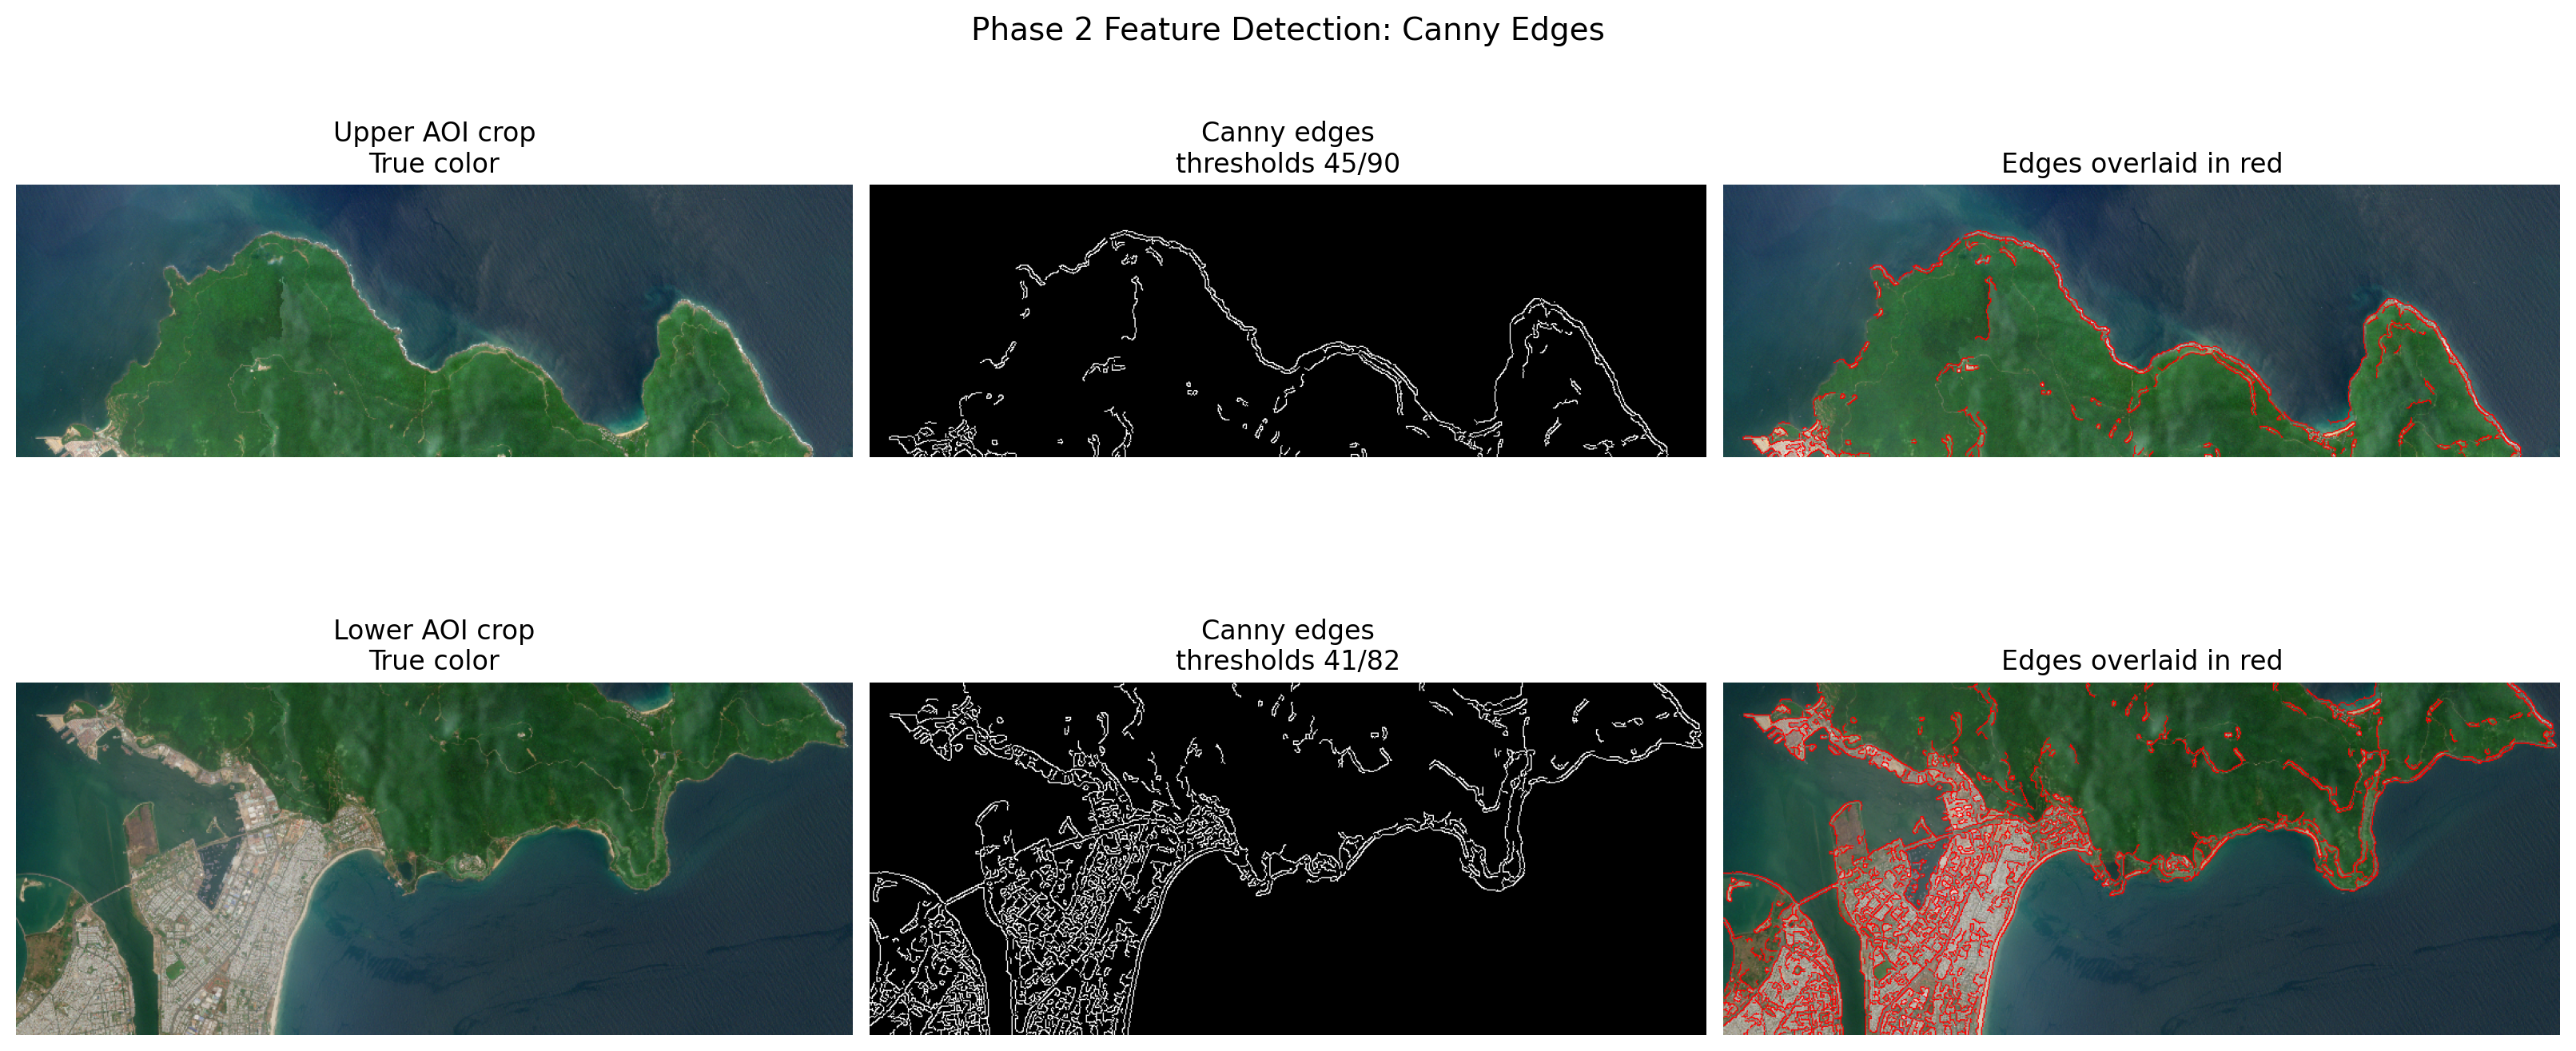
\includegraphics[width=0.48\textwidth]{../output/phase2_canny_edges_2024.png}
    \hfill
    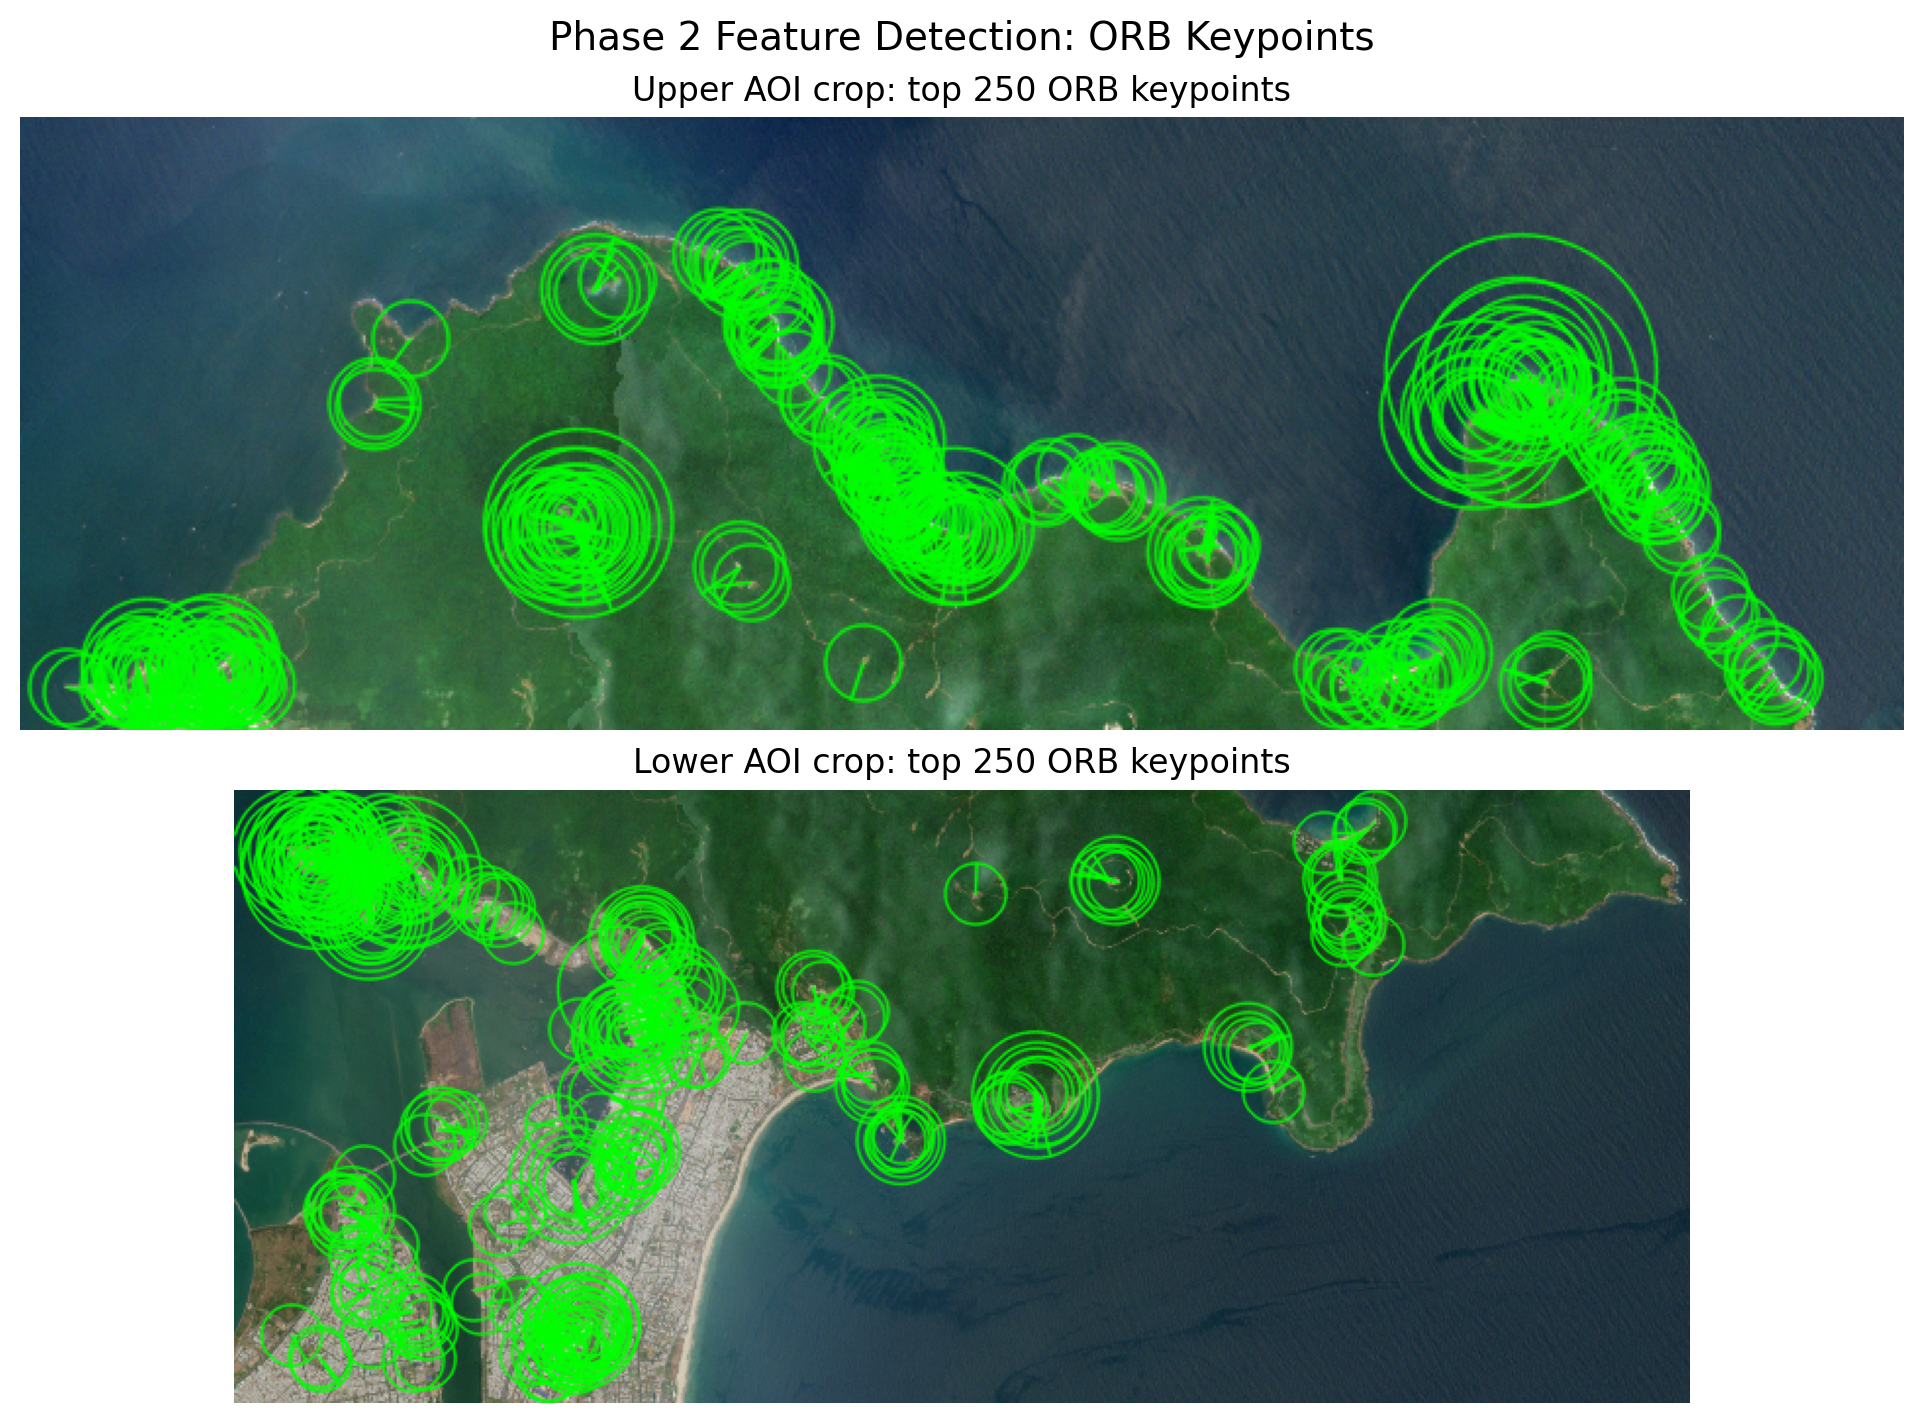
\includegraphics[width=0.48\textwidth]{../output/phase2_orb_keypoints_2024.png}
    \caption{Left: Canny edge detection highlighting structural boundaries. Right: ORB keypoints clustering over highly textured urban and industrial zones.}
    \label{fig:phase2_features}
\end{figure}

\subsection{Land-Cover Segmentation}
To group pixels into meaningful land-cover classes, we utilized the \textbf{Mean Shift} segmentation algorithm on the true-color imagery. Mean Shift is a non-parametric clustering technique that effectively smooths local color variations and merges similar pixels into homogeneous regions without requiring a predefined number of clusters. 
Following the clustering, we utilized the spectral indices computed in Phase 1 (NDVI and NDWI) to assign semantic labels to the segmented regions (e.g., Vegetation, Water, Built-up/Barren).

\begin{figure}[H]
    \centering
    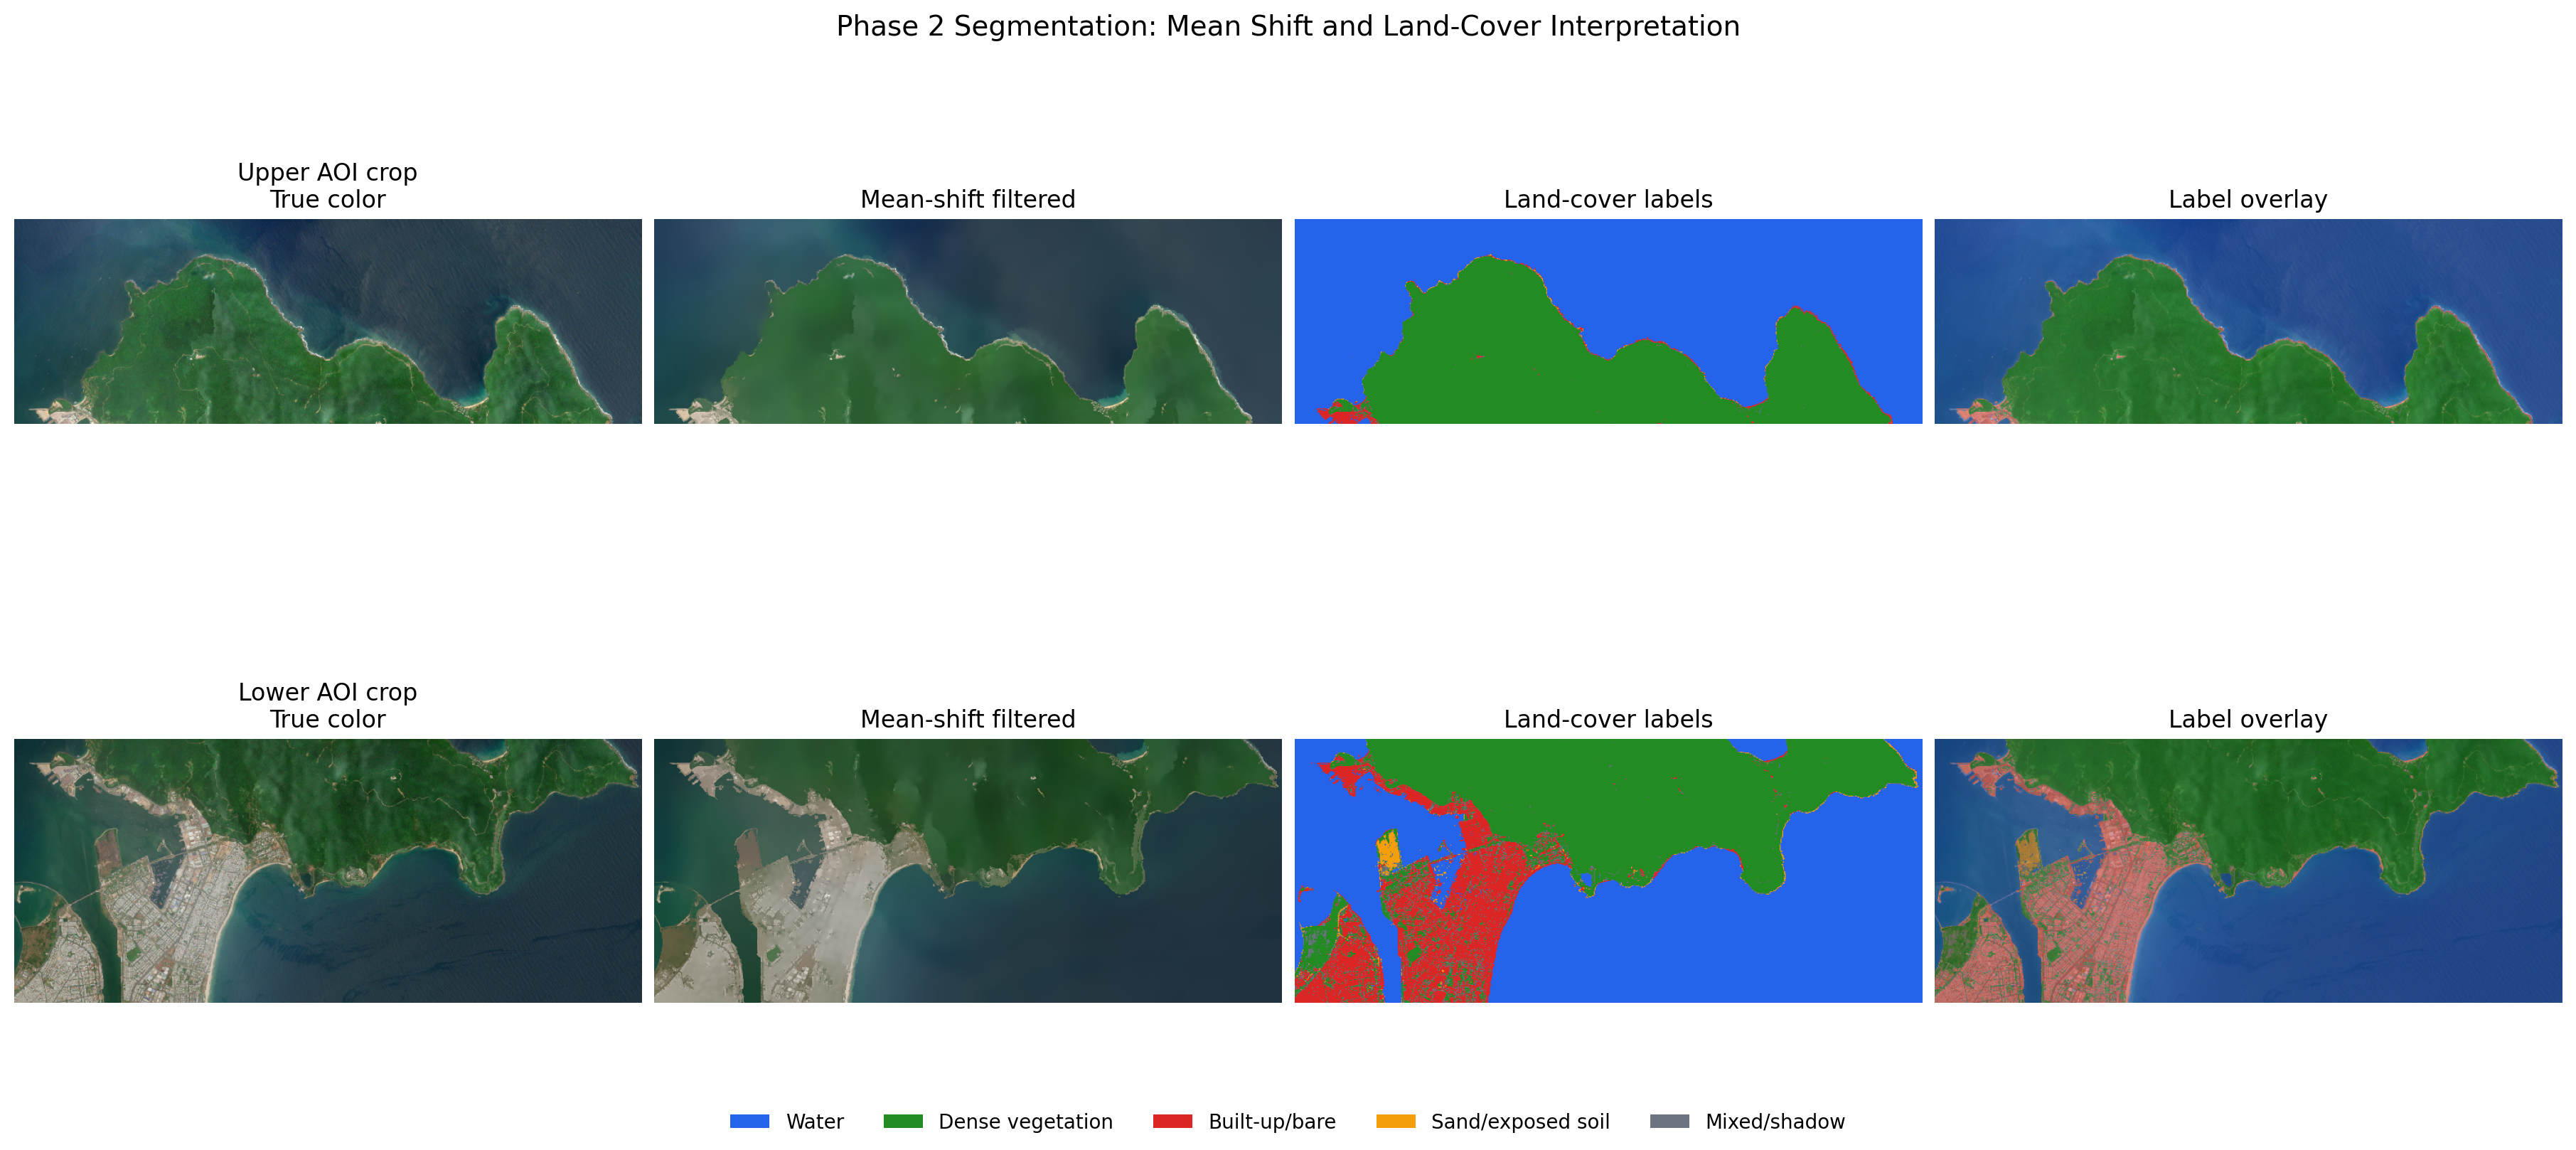
\includegraphics[width=0.98\textwidth]{../output/phase2_mean_shift_landcover_segmentation_2024.png}
    \caption{Mean Shift segmentation results assigning distinct color labels to different land-cover categories based on spectral characteristics.}
    \label{fig:phase2_segmentation}
\end{figure}

\subsection{Sanity-Check Validation}
Due to the absence of ground-truth labeled datasets, we conducted a qualitative sanity-check validation by comparing our segmentation output against an OpenStreetMap (OSM) satellite basemap for the exact same region.

\begin{figure}[H]
    \centering
    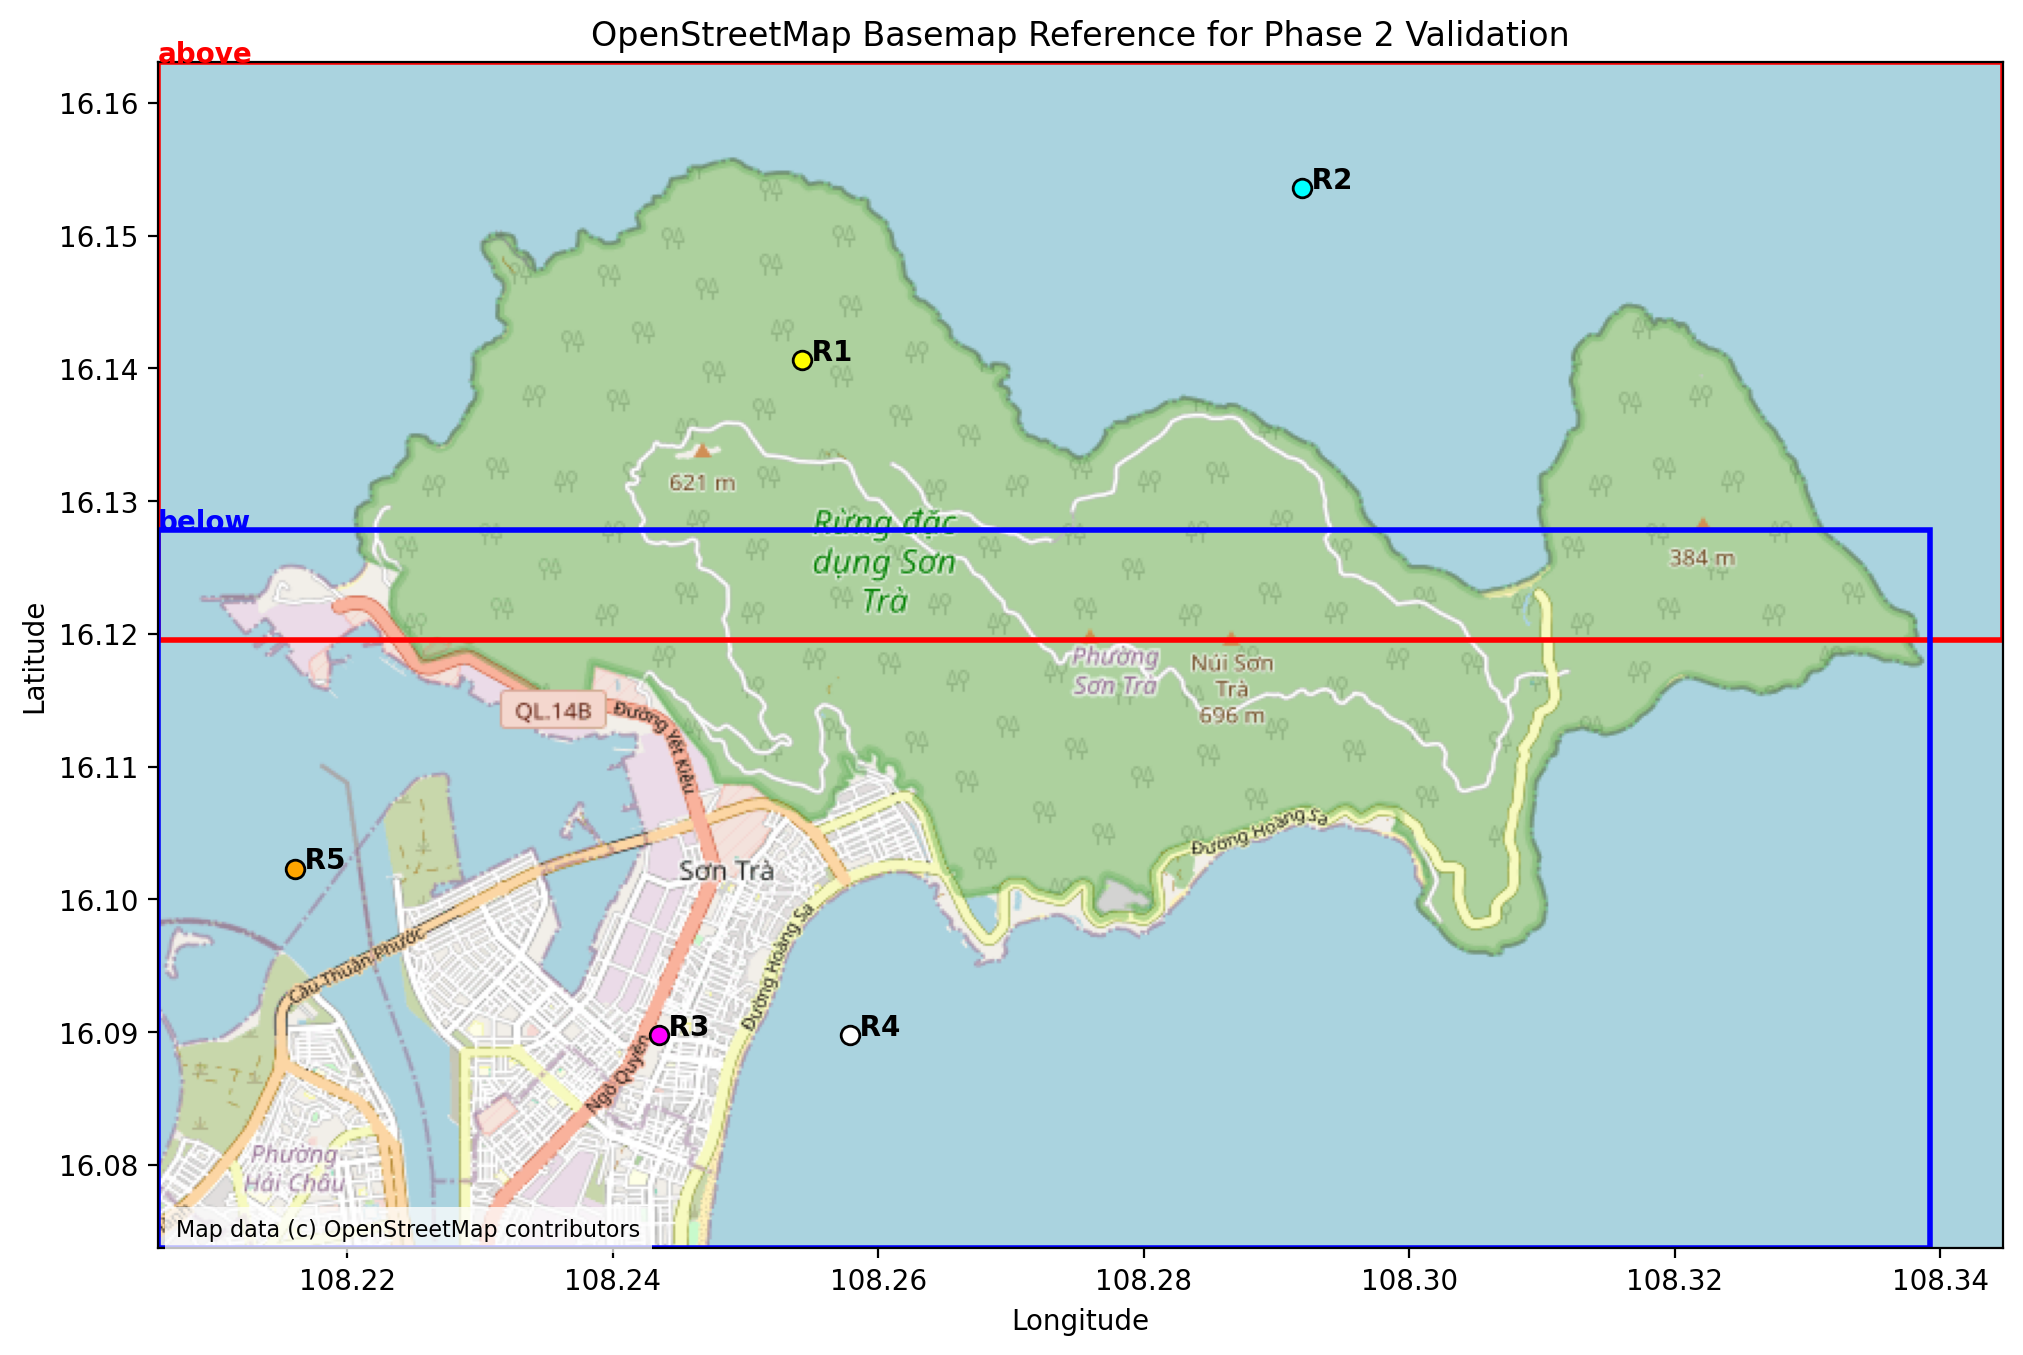
\includegraphics[width=0.98\textwidth]{../output/phase2_osm_basemap_reference.png}
    \caption{OpenStreetMap (OSM) Basemap serving as our reference ground-truth for qualitative validation. This high-resolution context allows us to visually pinpoint specific land-cover types prior to evaluating the algorithm's performance.}
    \label{fig:phase2_osm_reference}
\end{figure}

\begin{figure}[H]
    \centering
    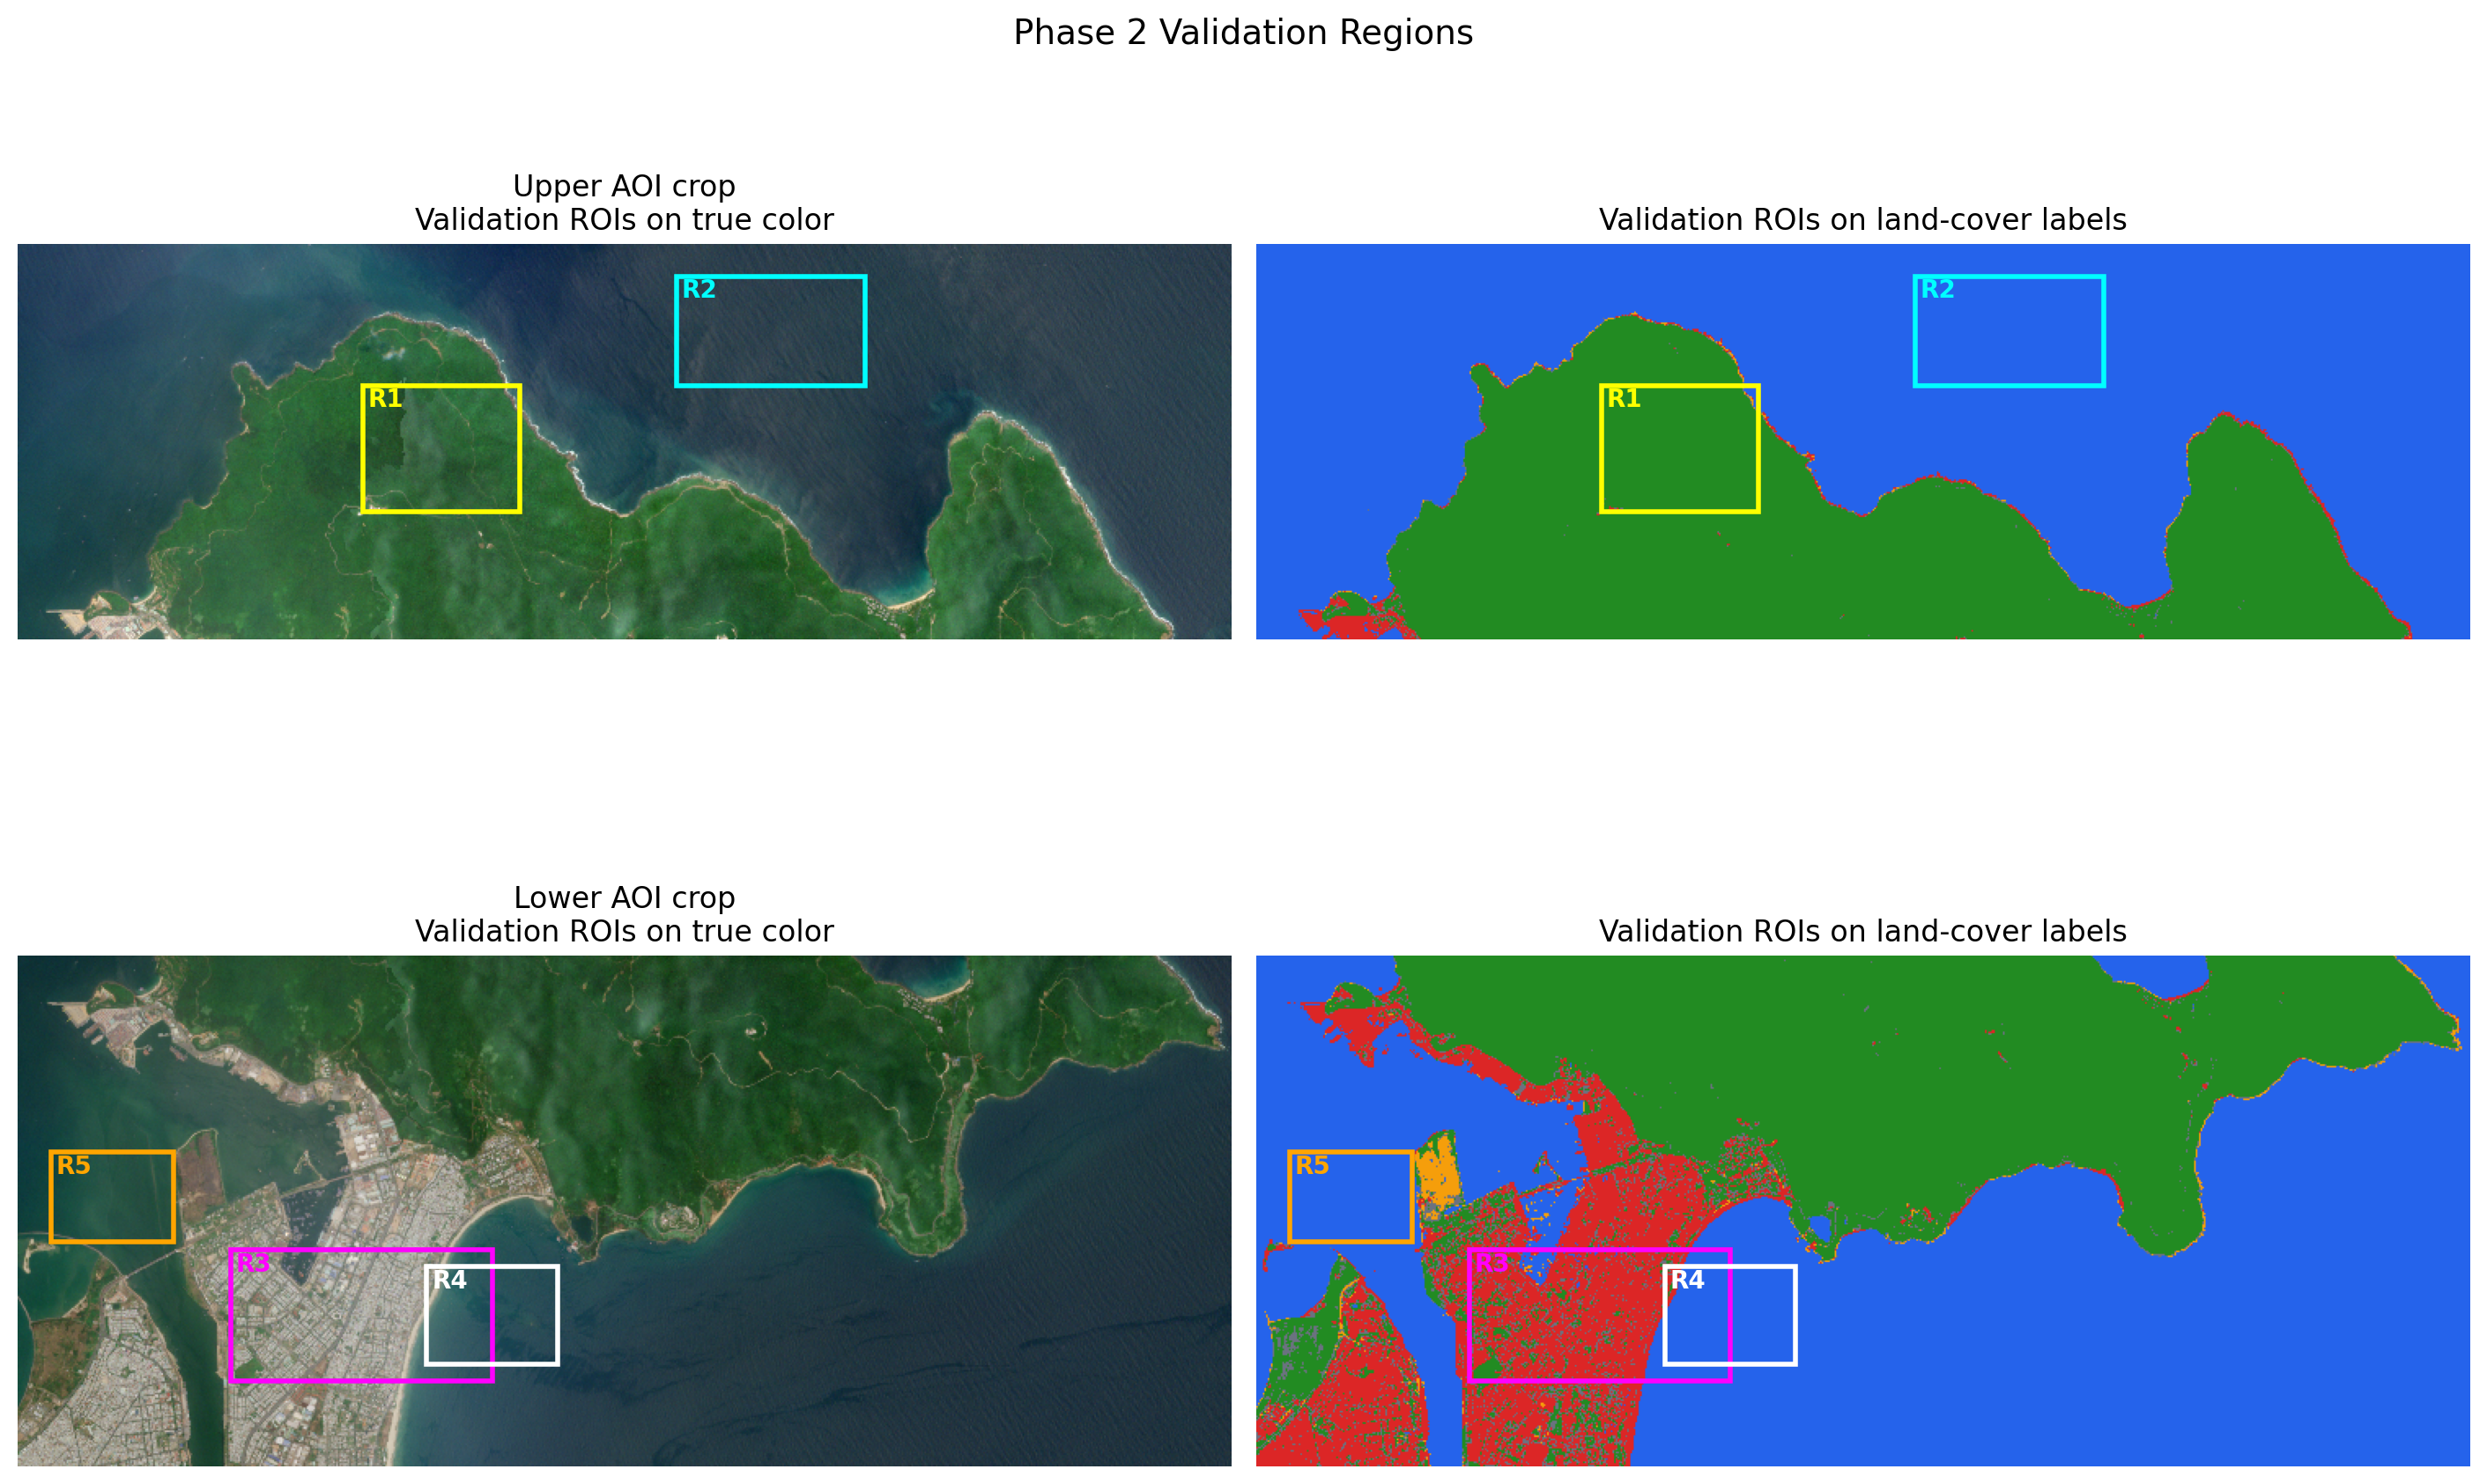
\includegraphics[width=0.98\textwidth]{../output/phase2_validation_regions_2024.png}
    \caption{Validation regions comparing our Mean Shift segmentation against the OSM Basemap.}
    \label{fig:phase2_validation}
\end{figure}

\textbf{Validation Findings:}
\begin{itemize}
    \item \textbf{Matches:} The algorithm successfully isolated large, distinct topographical features. The ocean/coastline boundary was segmented perfectly due to its strong spectral divergence from the sandy beach. Similarly, dense forests (high NDVI) were accurately clustered.
    \item \textbf{Limitations/Mismatches:} The algorithm struggled to differentiate between bare soil/sand and concrete infrastructure, clustering them into the same "Built-up/Barren" class. This occurs because both materials exhibit similar reflectance profiles in the visible spectrum. Additionally, very small urban patches (e.g., narrow tree-lined streets) were absorbed into the surrounding urban clusters due to the spatial resolution ($10\text{ m/pixel}$) limitations of the Sentinel-2 data.
\end{itemize}

\section{Phase 3: Alignment \& Stitching}
In this phase, we tackle two core spatial operations using feature-based alignment: co-registering the 2026 temporal images onto the 2024 reference frame, and stitching the split Area of Interest (AOI) exports (the upper and lower crops) into a seamless mosaic.

\subsection{Methodology}
Both operations utilized the same computer vision pipeline for image registration:
\begin{enumerate}
    \item \textbf{Feature Detection and Matching:} We utilized the Scale-Invariant Feature Transform (SIFT) algorithm to detect distinctive keypoints and extract local descriptors from the grayscale-equalized images. The descriptors were then matched using a K-Nearest Neighbors (KNN) matcher combined with Lowe's ratio test to reject ambiguous matches.
    \item \textbf{Homography Estimation:} We applied the RANdom SAmple Consensus (RANSAC) algorithm to compute the $3 \times 3$ projective transformation matrix (homography) while robustly filtering out geometric outliers.
    \item \textbf{Image Warping and Blending:} Finally, the moving image was geometrically warped via perspective transformation. For the stitching process, a distance-transform-based feather blending algorithm was implemented to seamlessly merge the overlapping regions.
\end{enumerate}

\subsection{Temporal Co-registration (2026 to 2024)}
To ensure pixel-to-pixel spatial alignment for change detection, we mapped the 2026 imagery into the coordinate space of the 2024 reference date. 

\begin{figure}[H]
    \centering
    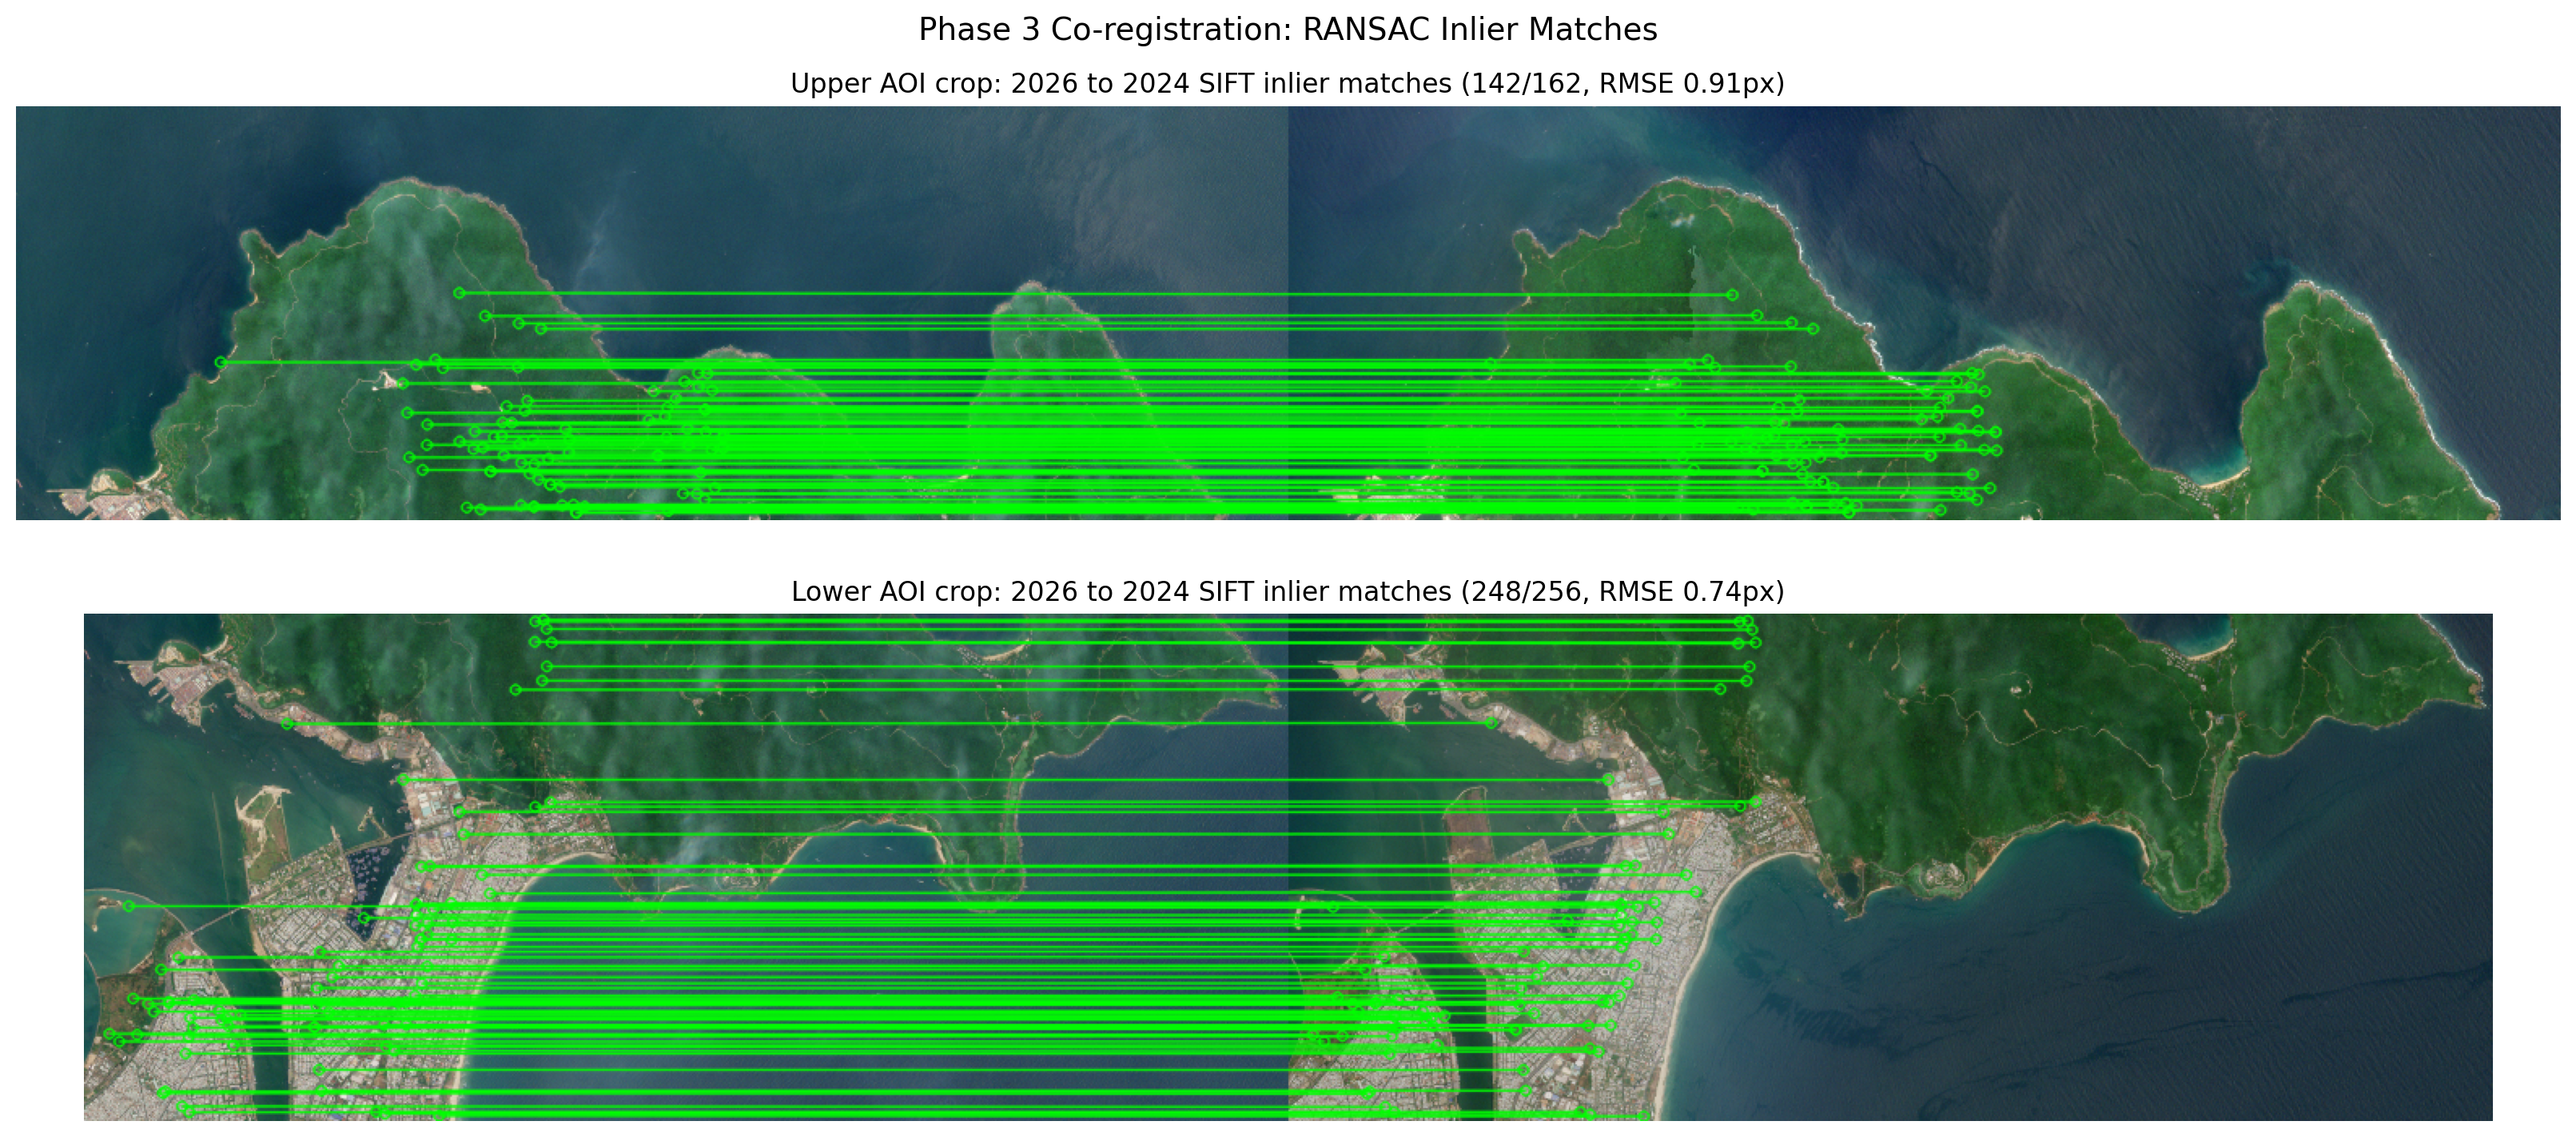
\includegraphics[width=0.98\textwidth]{../output/phase3_coregistration_matches_2026_to_2024.png}
    \caption{SIFT keypoint matches between the 2026 (moving) and 2024 (fixed) images. The green lines denote geometric inliers retained by RANSAC.}
    \label{fig:phase3_coregistration_matches}
\end{figure}

The co-registration achieved sub-pixel accuracy, significantly minimizing spatial misalignments. The Root Mean Square Error (RMSE) of the reprojected inliers was $0.908\text{ px}$ for the upper crop and $0.742\text{ px}$ for the lower crop.

\begin{figure}[H]
    \centering
    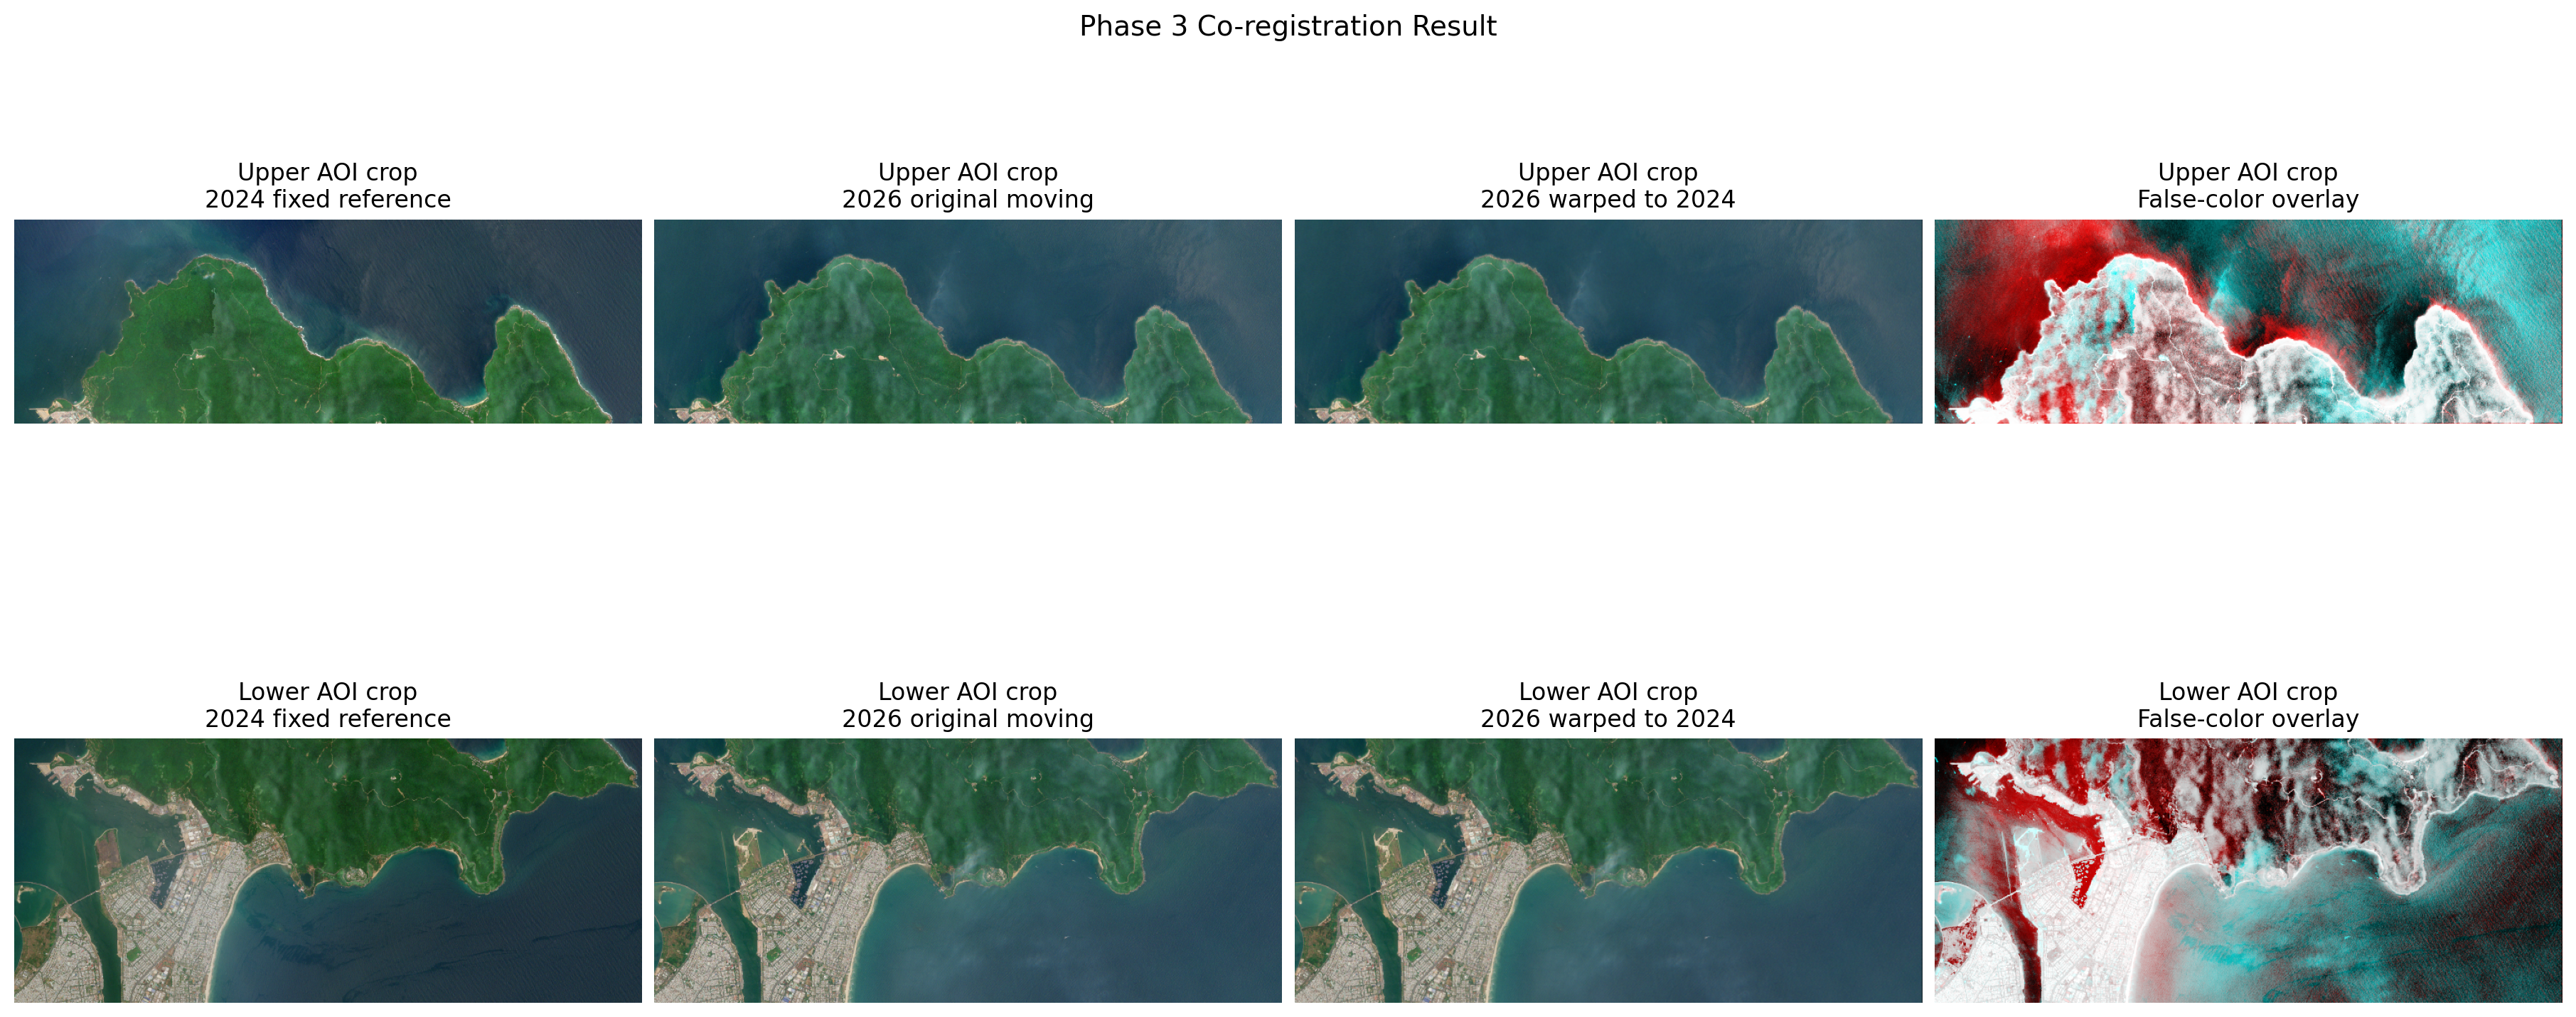
\includegraphics[width=0.98\textwidth]{../output/phase3_coregistration_comparison_2026_to_2024.png}
    \caption{Visual comparison of the 2026 imagery before and after co-registration onto the 2024 reference frame.}
    \label{fig:phase3_coregistration_comparison}
\end{figure}

To demonstrate the critical necessity of this step, we computed the absolute pixel difference between the 2024 and 2026 images before and after alignment. Without co-registration, the slight orbital offset produces severe "ghosting" artifacts along structural edges (false changes). After alignment, these artifacts are drastically reduced, ensuring that any remaining pixel differences represent genuine land-cover changes for Phase 4.

\begin{figure}[H]
    \centering
    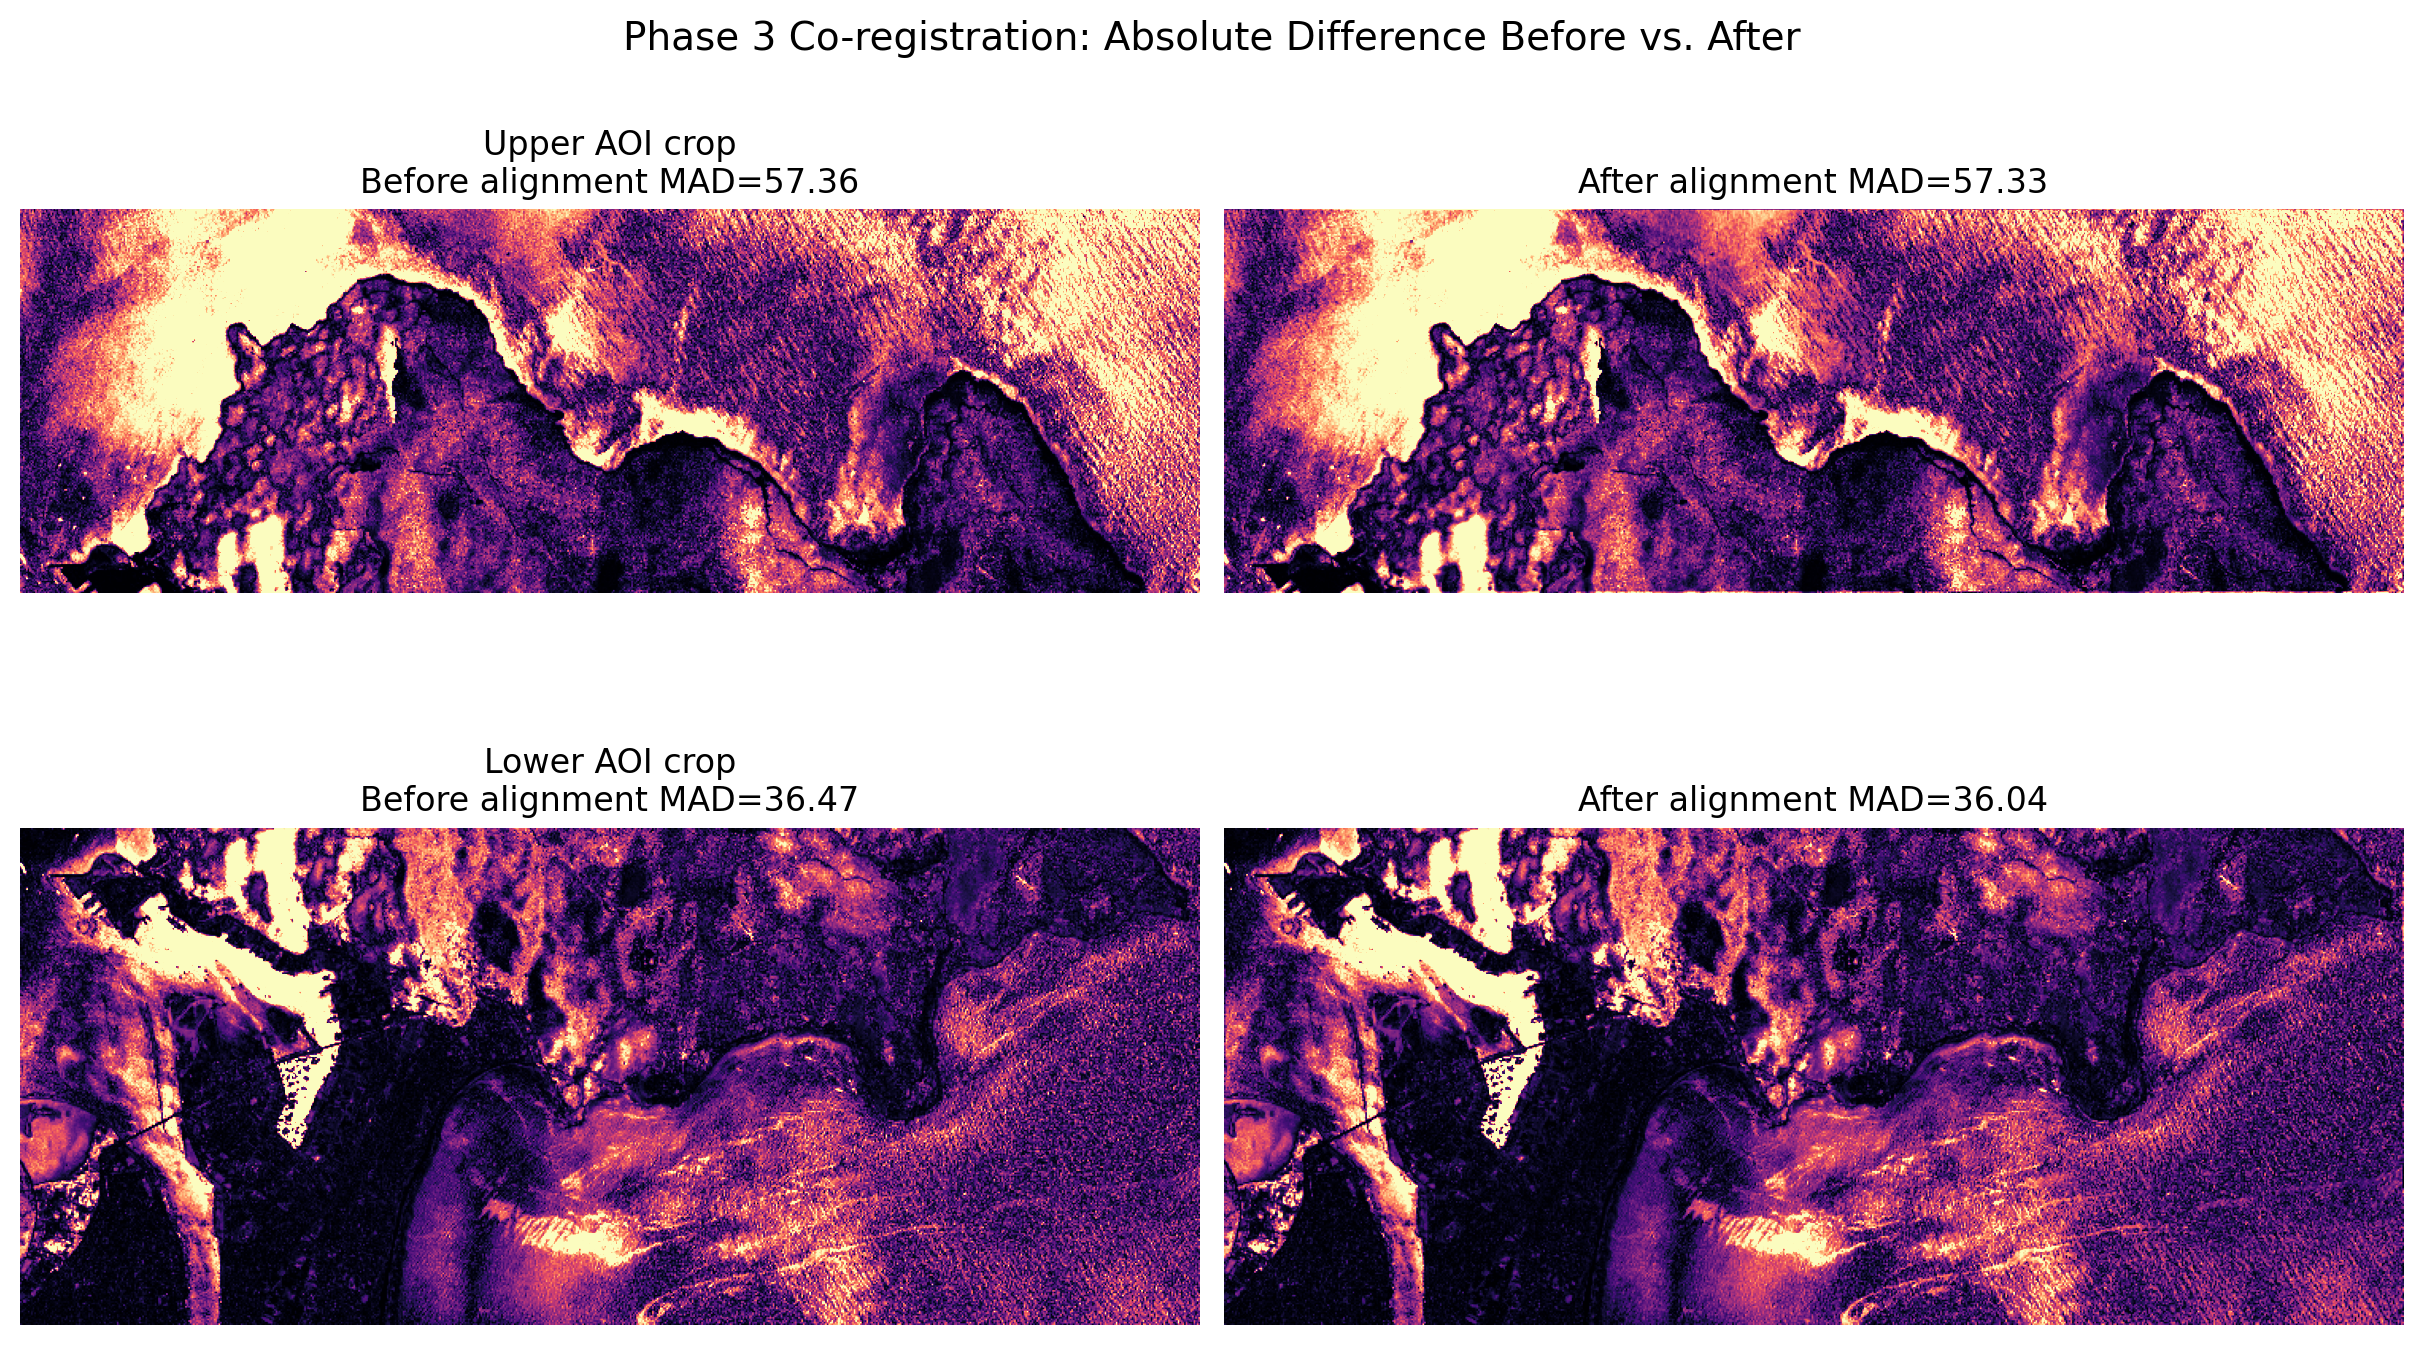
\includegraphics[width=0.98\textwidth]{../output/phase3_coregistration_difference_before_after.png}
    \caption{Absolute difference maps between 2024 and 2026. Left: Before alignment, showing severe misregistration artifacts. Right: After alignment, with false-change artifacts eliminated.}
    \label{fig:phase3_coregistration_difference}
\end{figure}

\subsection{Image Stitching}
Using the exact same pipeline, we stitched the upper and lower AOI exports back together. The SIFT algorithm successfully matched keypoints in the overlapping intersection between the two images. 

\begin{figure}[H]
    \centering
    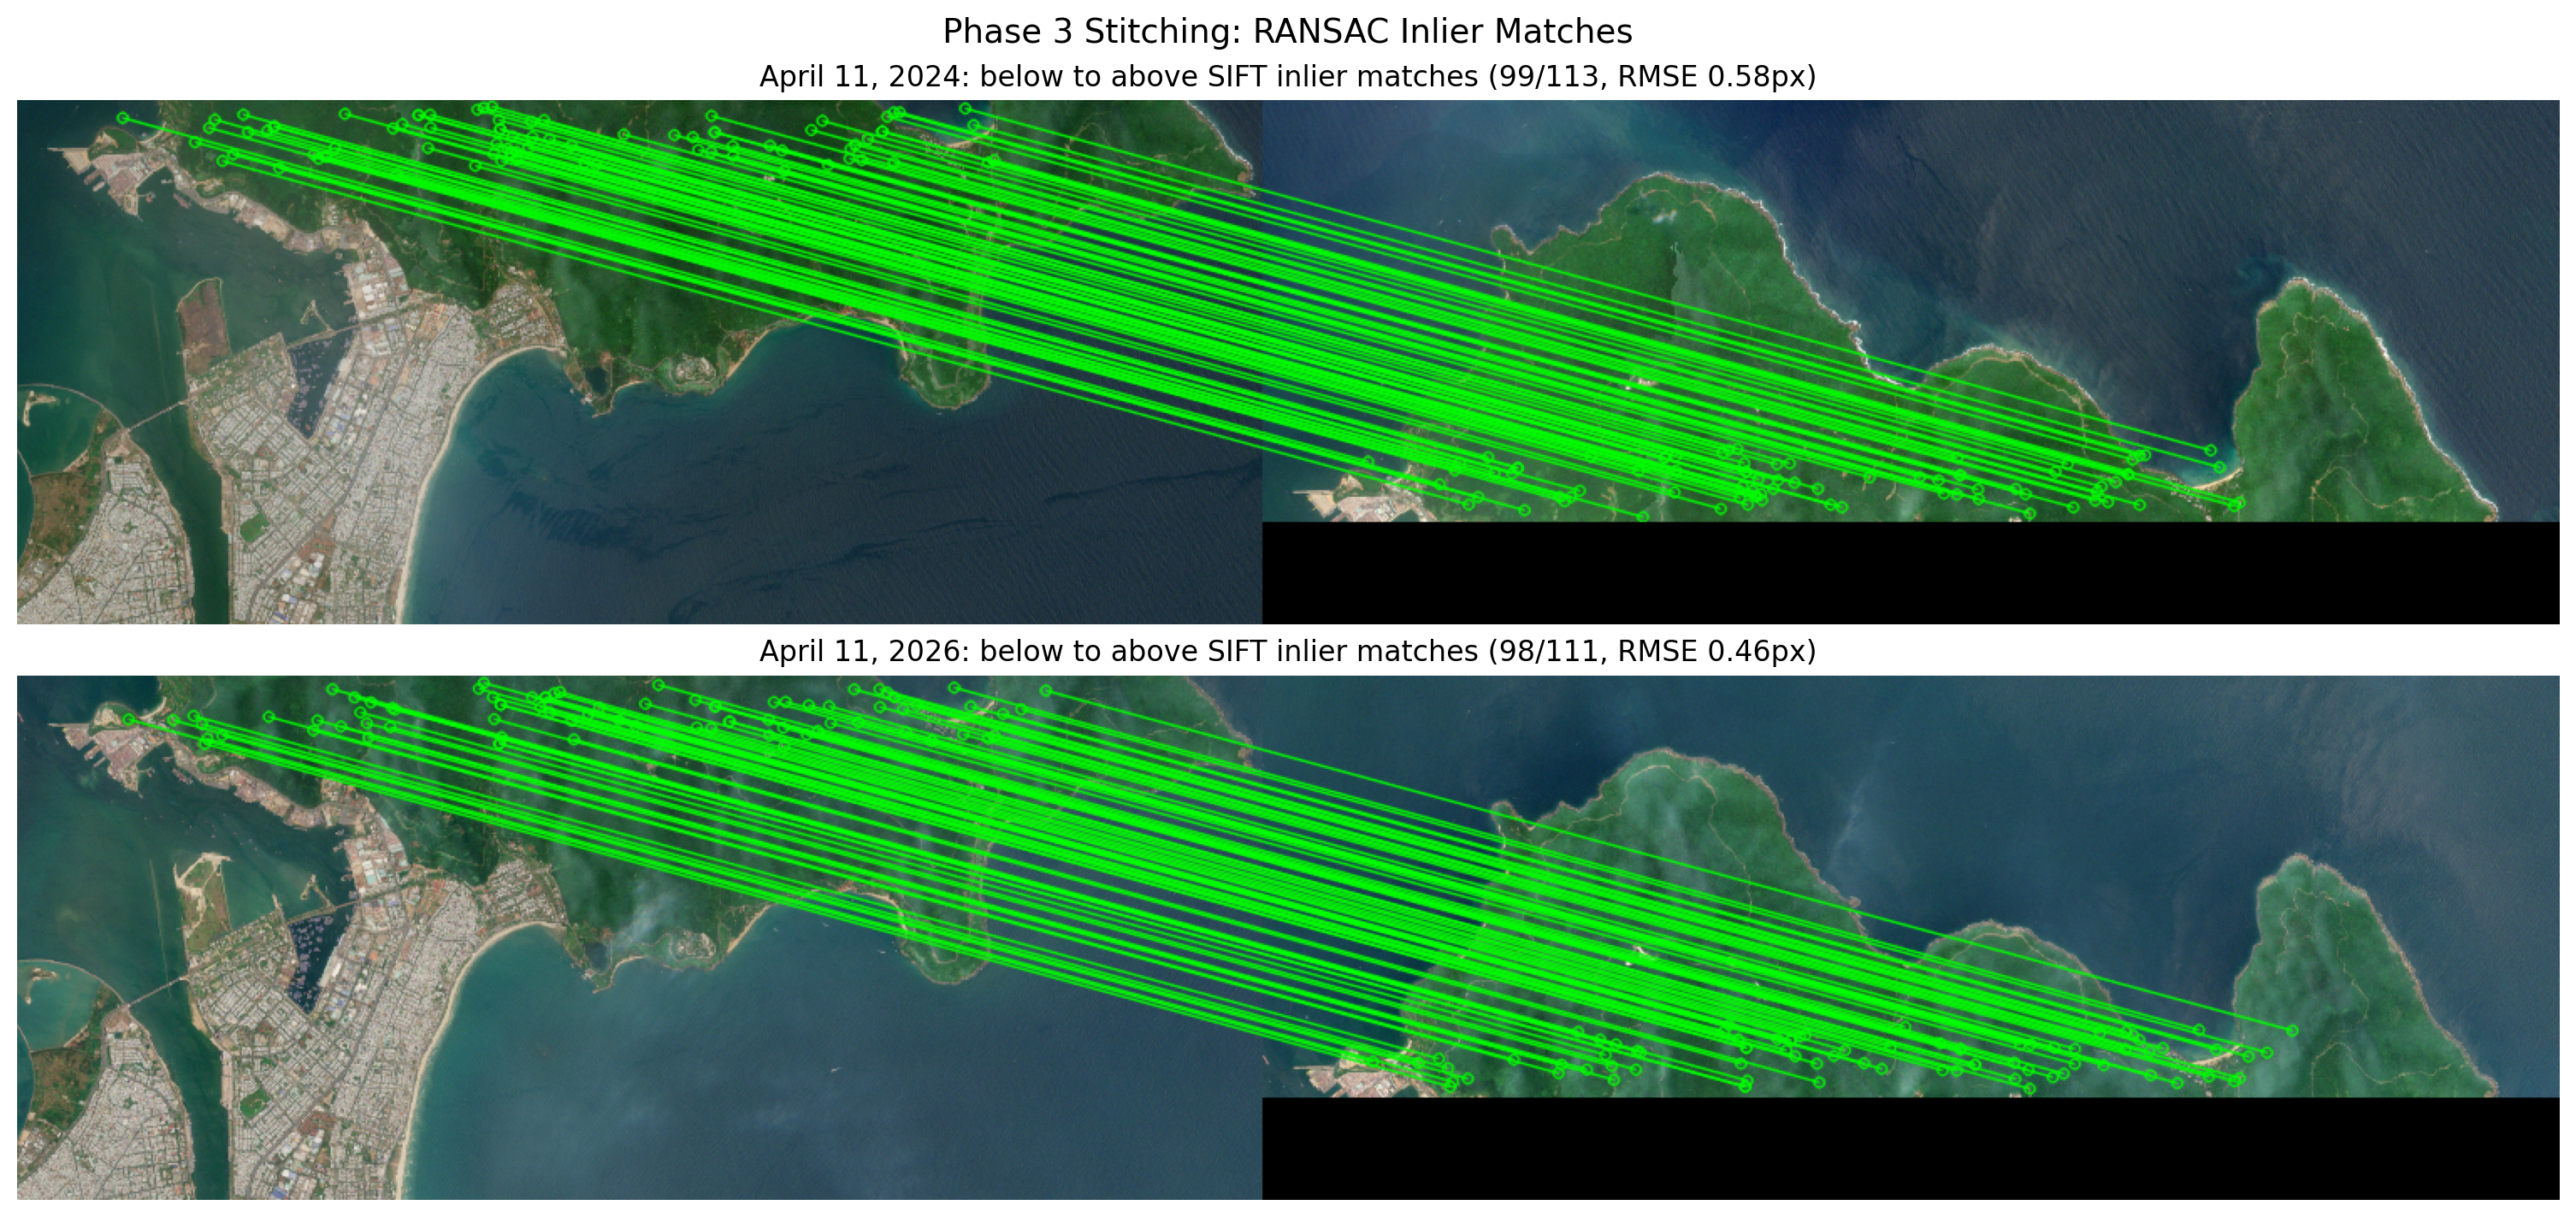
\includegraphics[width=0.98\textwidth]{../output/phase3_stitching_matches_above_below.png}
    \caption{SIFT keypoint matching between the upper and lower AOI crops, allowing for the estimation of the stitching homography.}
    \label{fig:phase3_stitching_matches}
\end{figure}

A distance-transform feather blending algorithm was then used to merge the crops, completely eliminating the visible seam line and restoring the full Area of Interest into a single continuous mosaic for both the 2024 and 2026 datasets.

\begin{figure}[H]
    \centering
    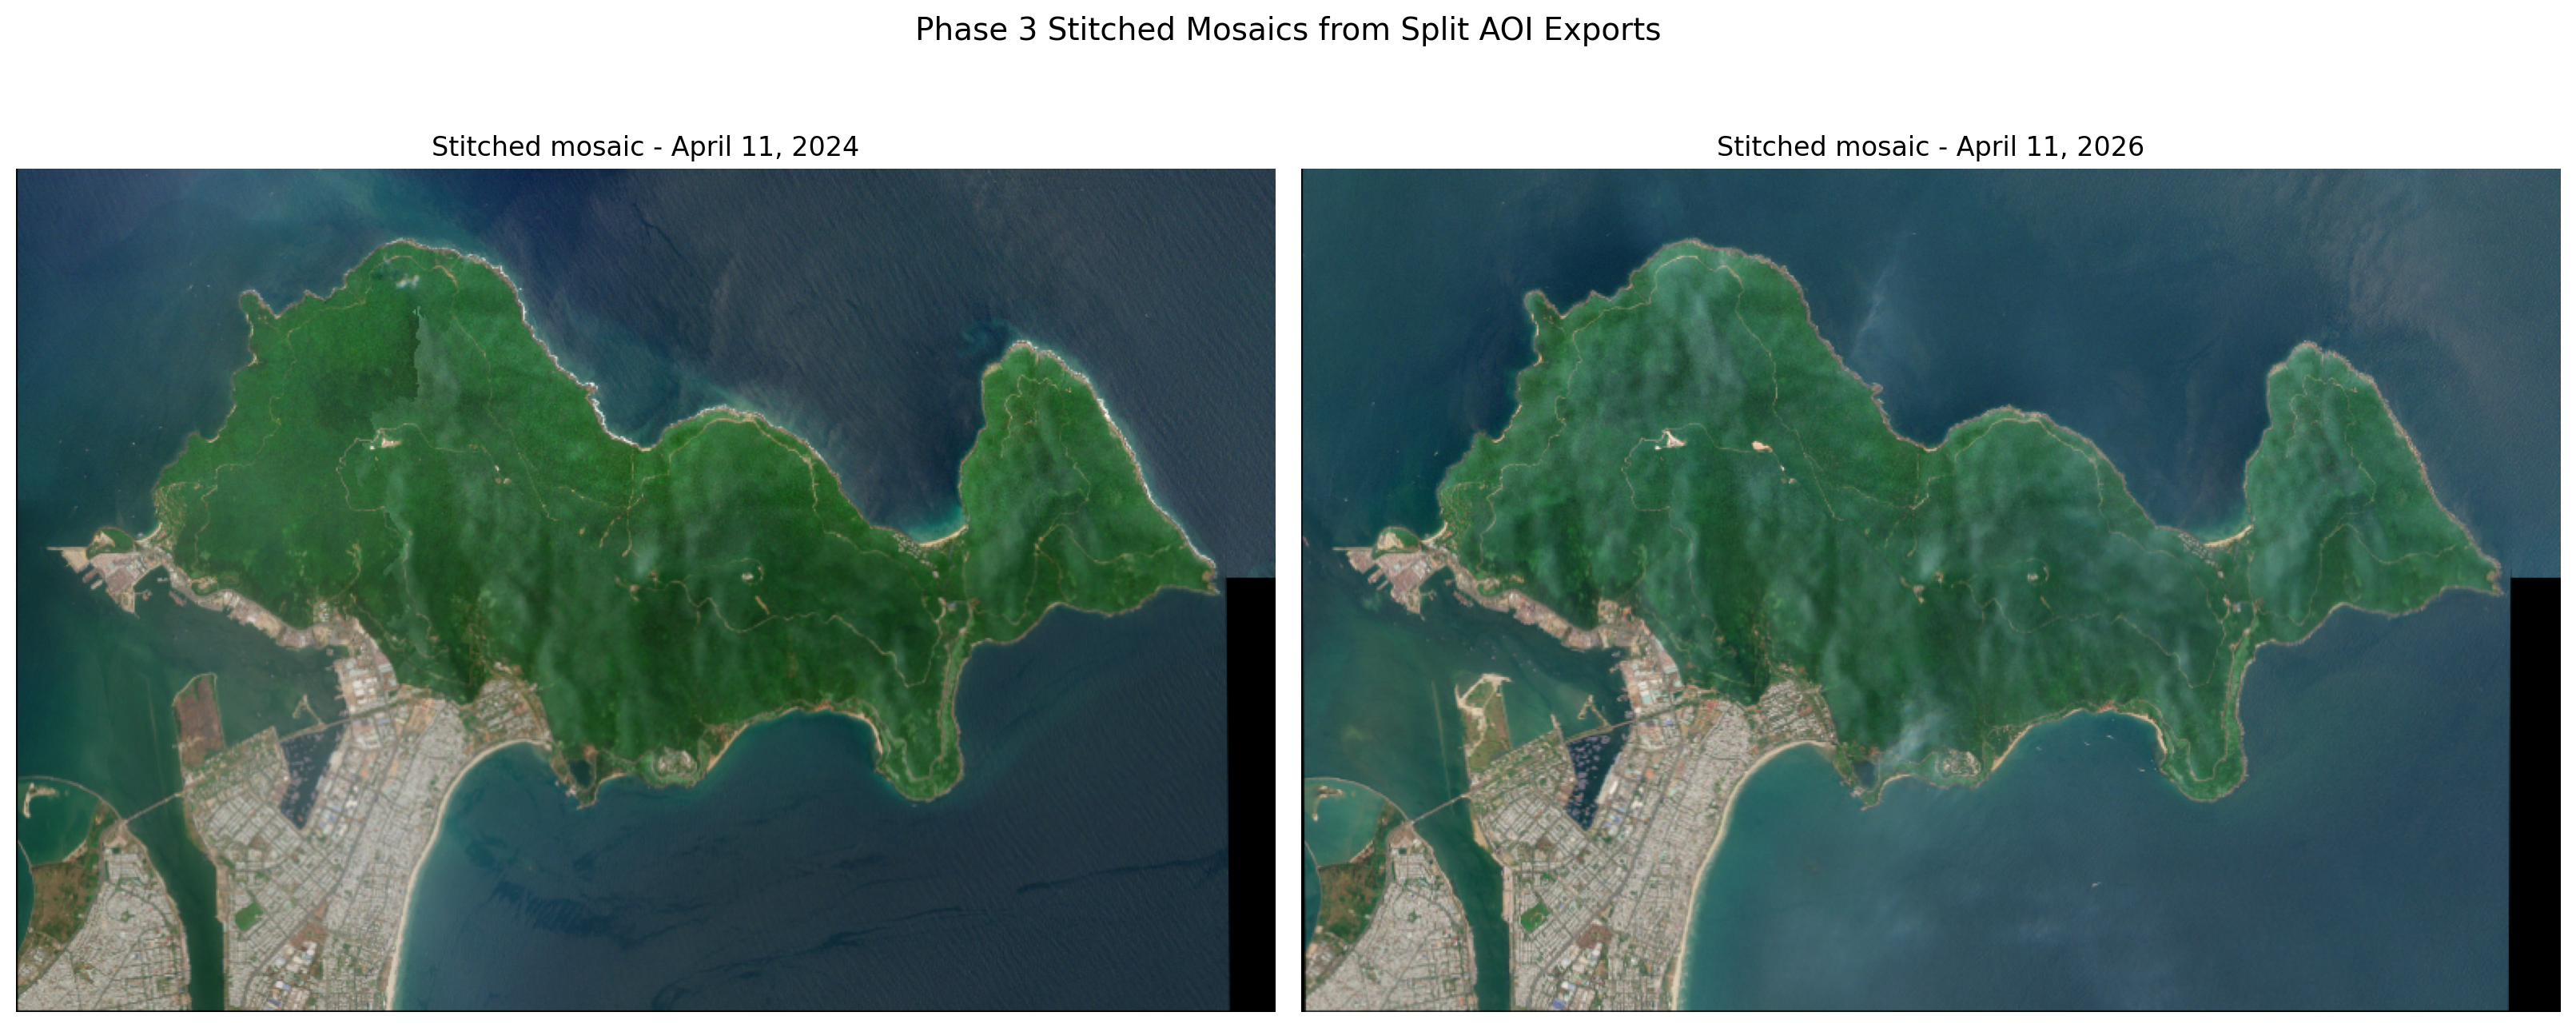
\includegraphics[width=0.98\textwidth]{../output/phase3_stitched_mosaics_comparison.png}
    \caption{Final stitched mosaics for the complete AOI in both 2024 and 2026, generated via feature-based alignment and feather blending.}
    \label{fig:phase3_stitched_mosaics}
\end{figure}

\section{Phase 4: Detection \& Change Tracking}
Building upon the segmentation logic and feature alignment established in earlier phases, this phase aims to automatically detect built-up urban infrastructure and track its expansion between 2024 and 2026.

\subsection{Object Detection: Built-up Regions}
To isolate built-up areas, we applied a multi-condition spectral classifier leveraging the NDVI, NDWI, and HSV color space (value and saturation). This classifier successfully isolated concrete, asphalt, and rooftops while rejecting vegetation, water, and sand. We applied morphological opening and closing to clean the binary mask and remove isolated pixel noise. 

\begin{figure}[H]
    \centering
    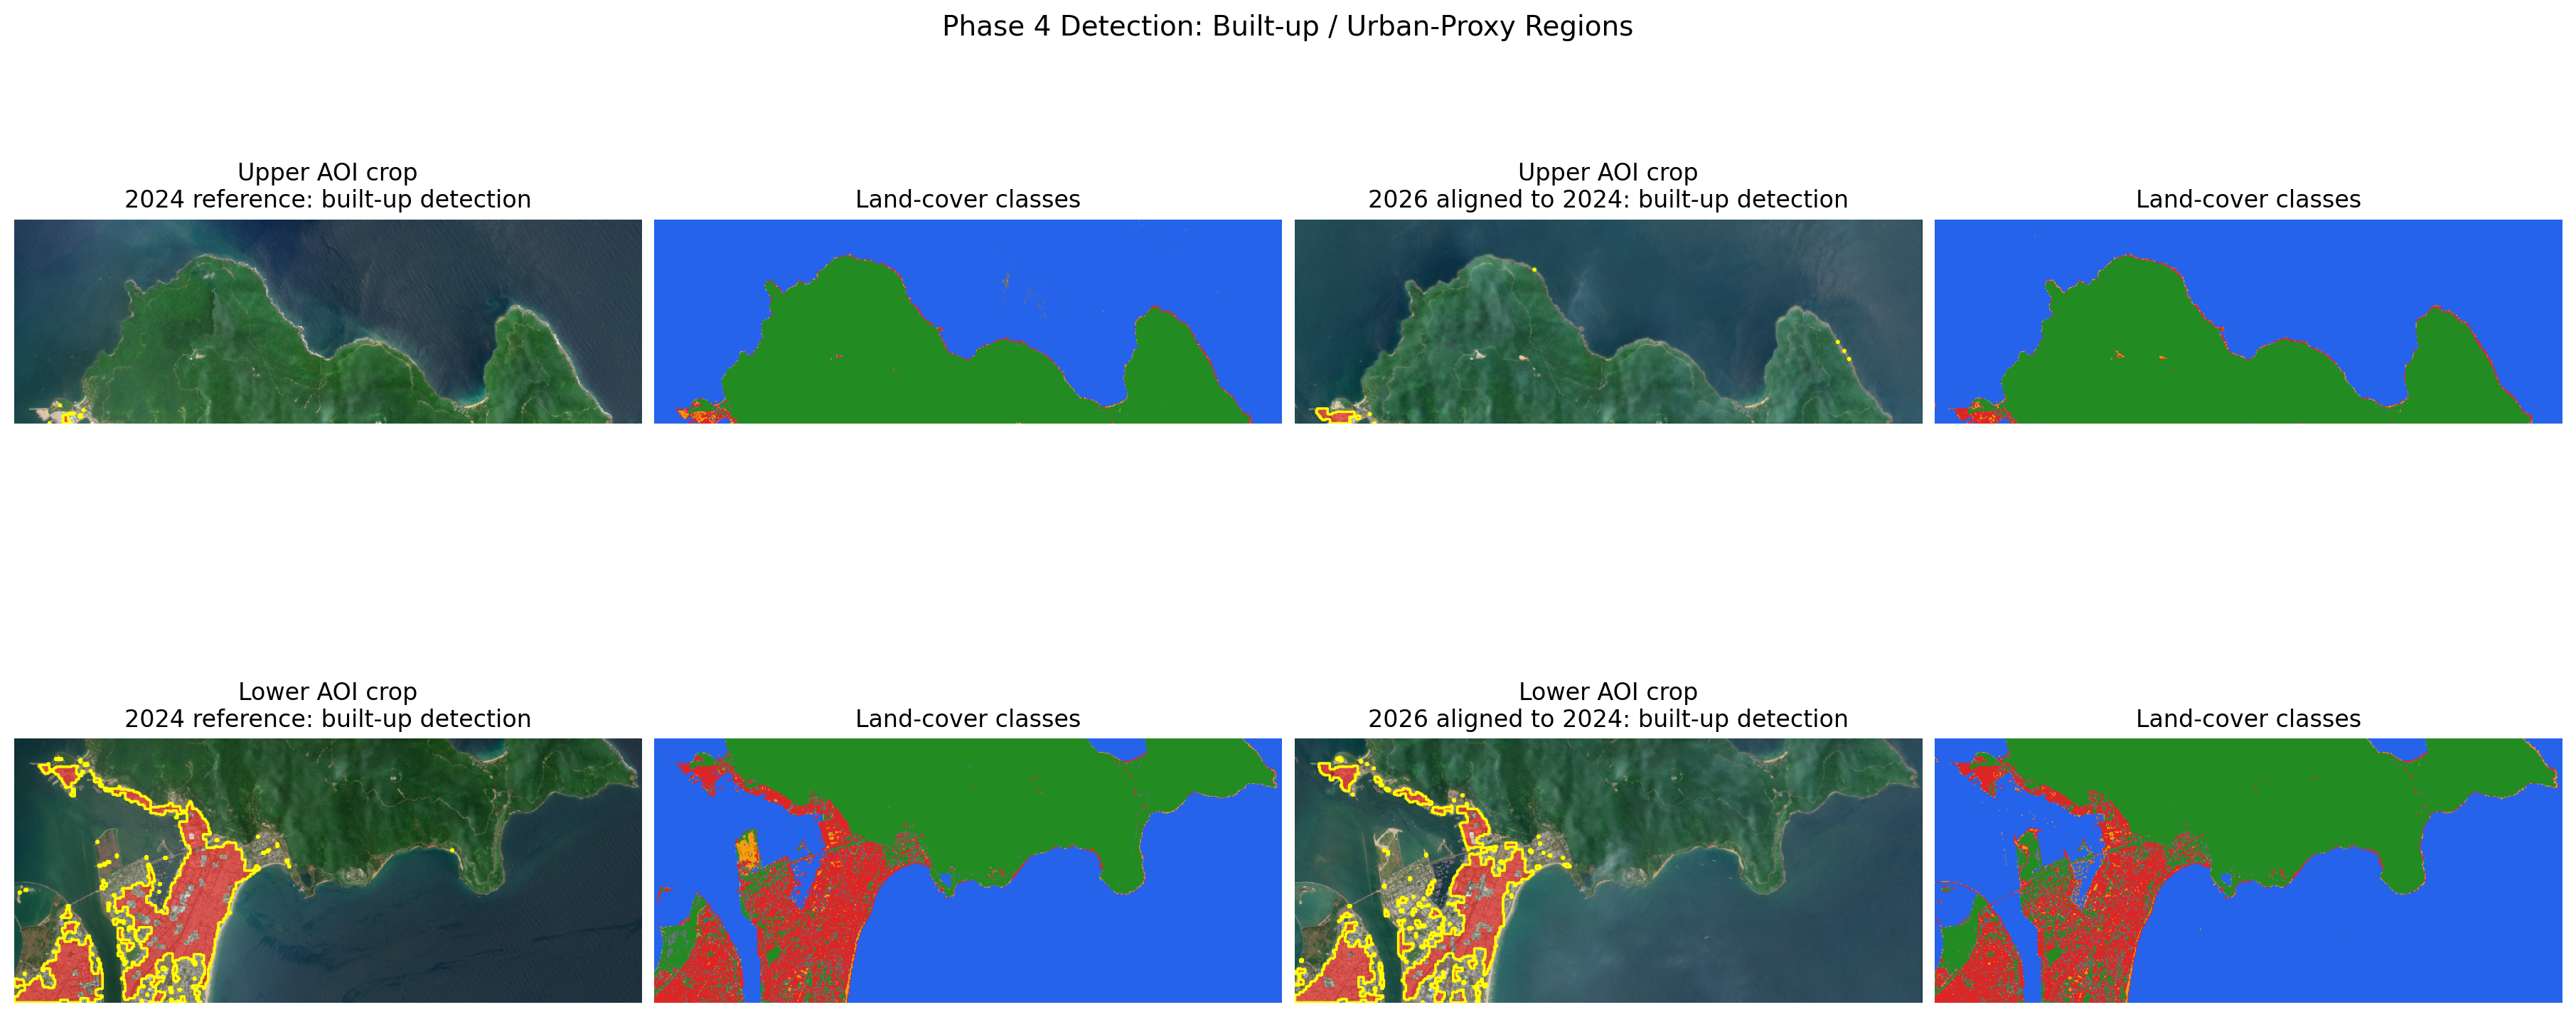
\includegraphics[width=0.98\textwidth]{../output/phase4_builtup_detection_2024_2026.png}
    \caption{Detection of built-up / urban proxy regions for both 2024 and the co-registered 2026 imagery.}
    \label{fig:phase4_builtup_detection}
\end{figure}

\subsection{Change Tracking}
Using the co-registered image pair, we computed a binary difference map of the built-up masks to highlight areas of new urban development. 

\begin{figure}[H]
    \centering
    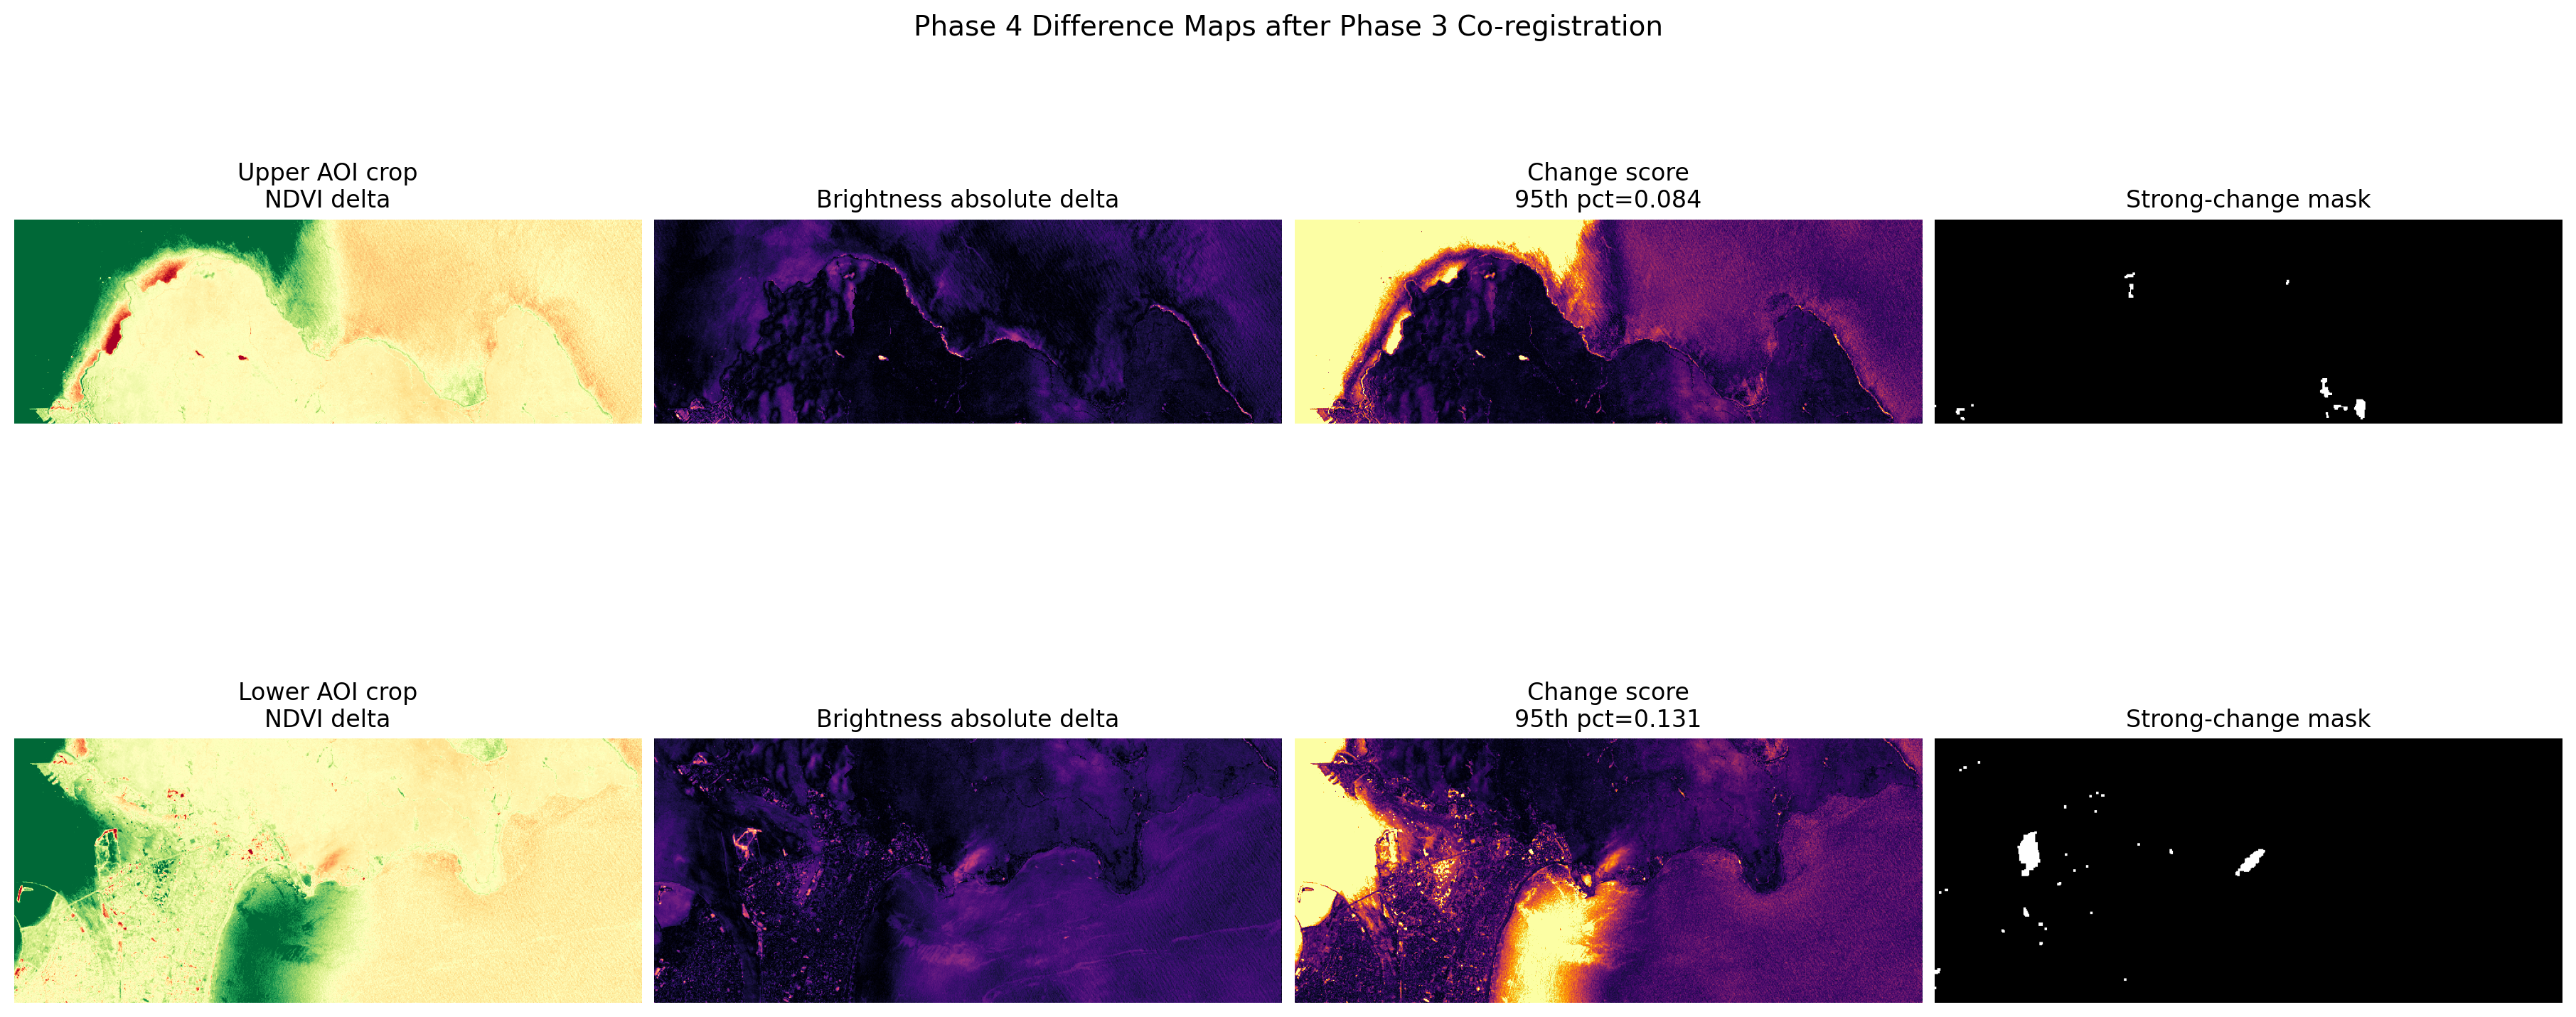
\includegraphics[width=0.98\textwidth]{../output/phase4_difference_maps.png}
    \caption{Binary difference maps highlighting raw pixel-level changes in built-up areas between 2024 and 2026.}
    \label{fig:phase4_difference_maps}
\end{figure}

To frame this as a spatial tracking problem, we extracted connected components from the difference map and outlined the largest changed regions using bounding boxes.

\begin{figure}[H]
    \centering
    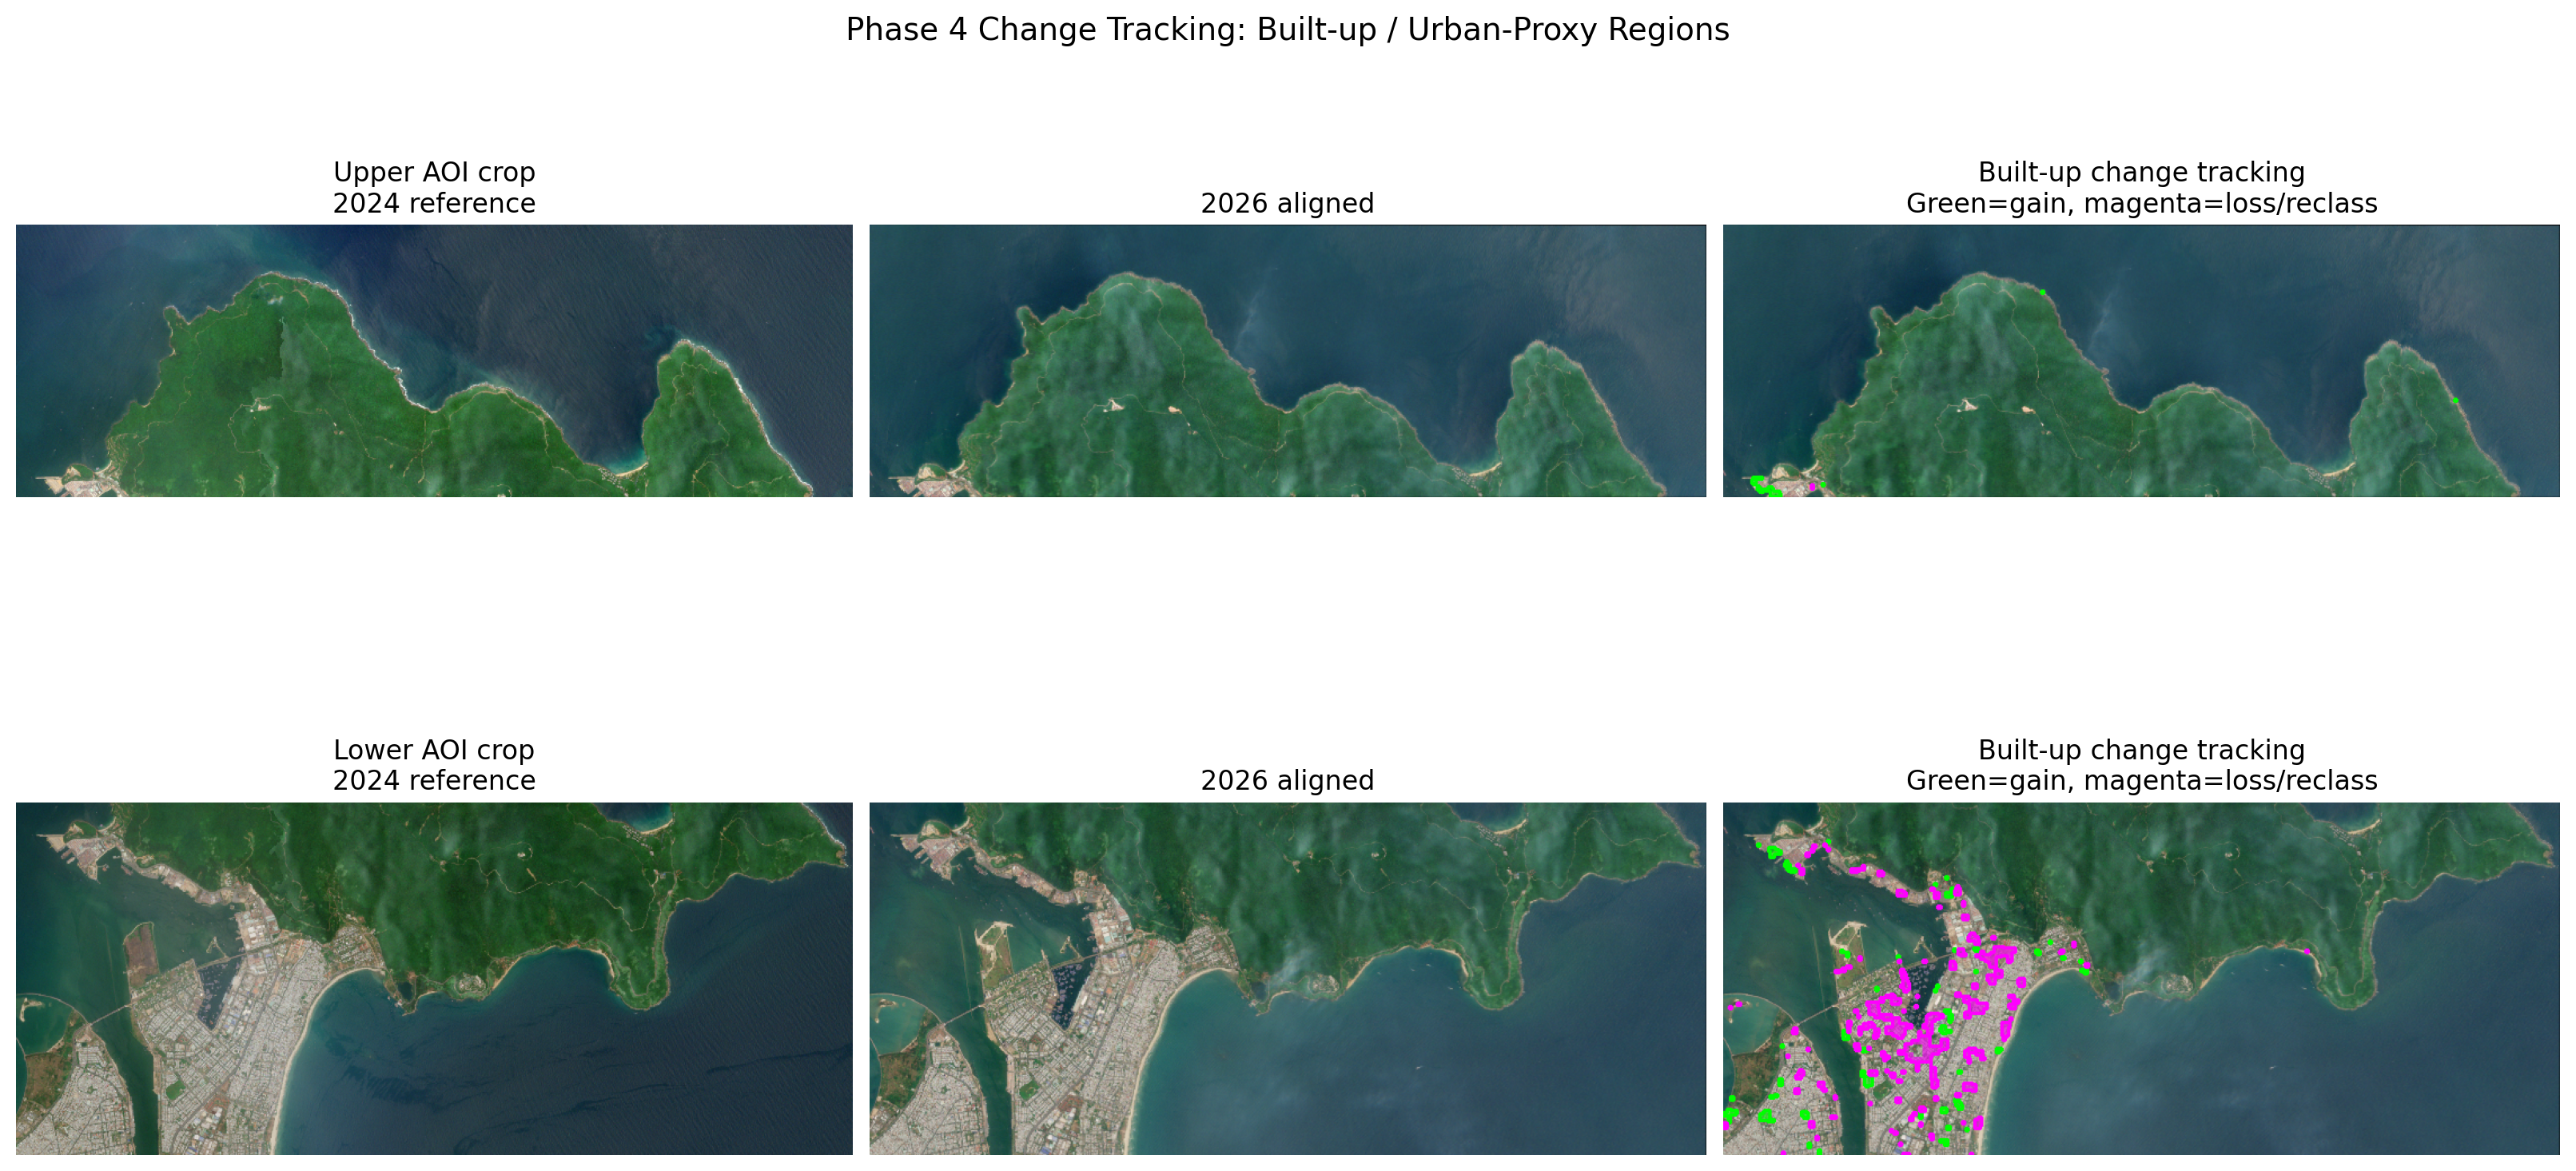
\includegraphics[width=0.98\textwidth]{../output/phase4_builtup_change_tracking.png}
    \caption{Change tracking of built-up areas. Red bounding boxes highlight the largest contiguous regions of newly detected urban infrastructure in 2026 compared to 2024.}
    \label{fig:phase4_builtup_change_tracking}
\end{figure}

The tracking results successfully pinpointed areas of major construction, such as new residential zoning, road expansions, and industrial land reclamation along the coastline and river deltas. 

\begin{figure}[H]
    \centering
    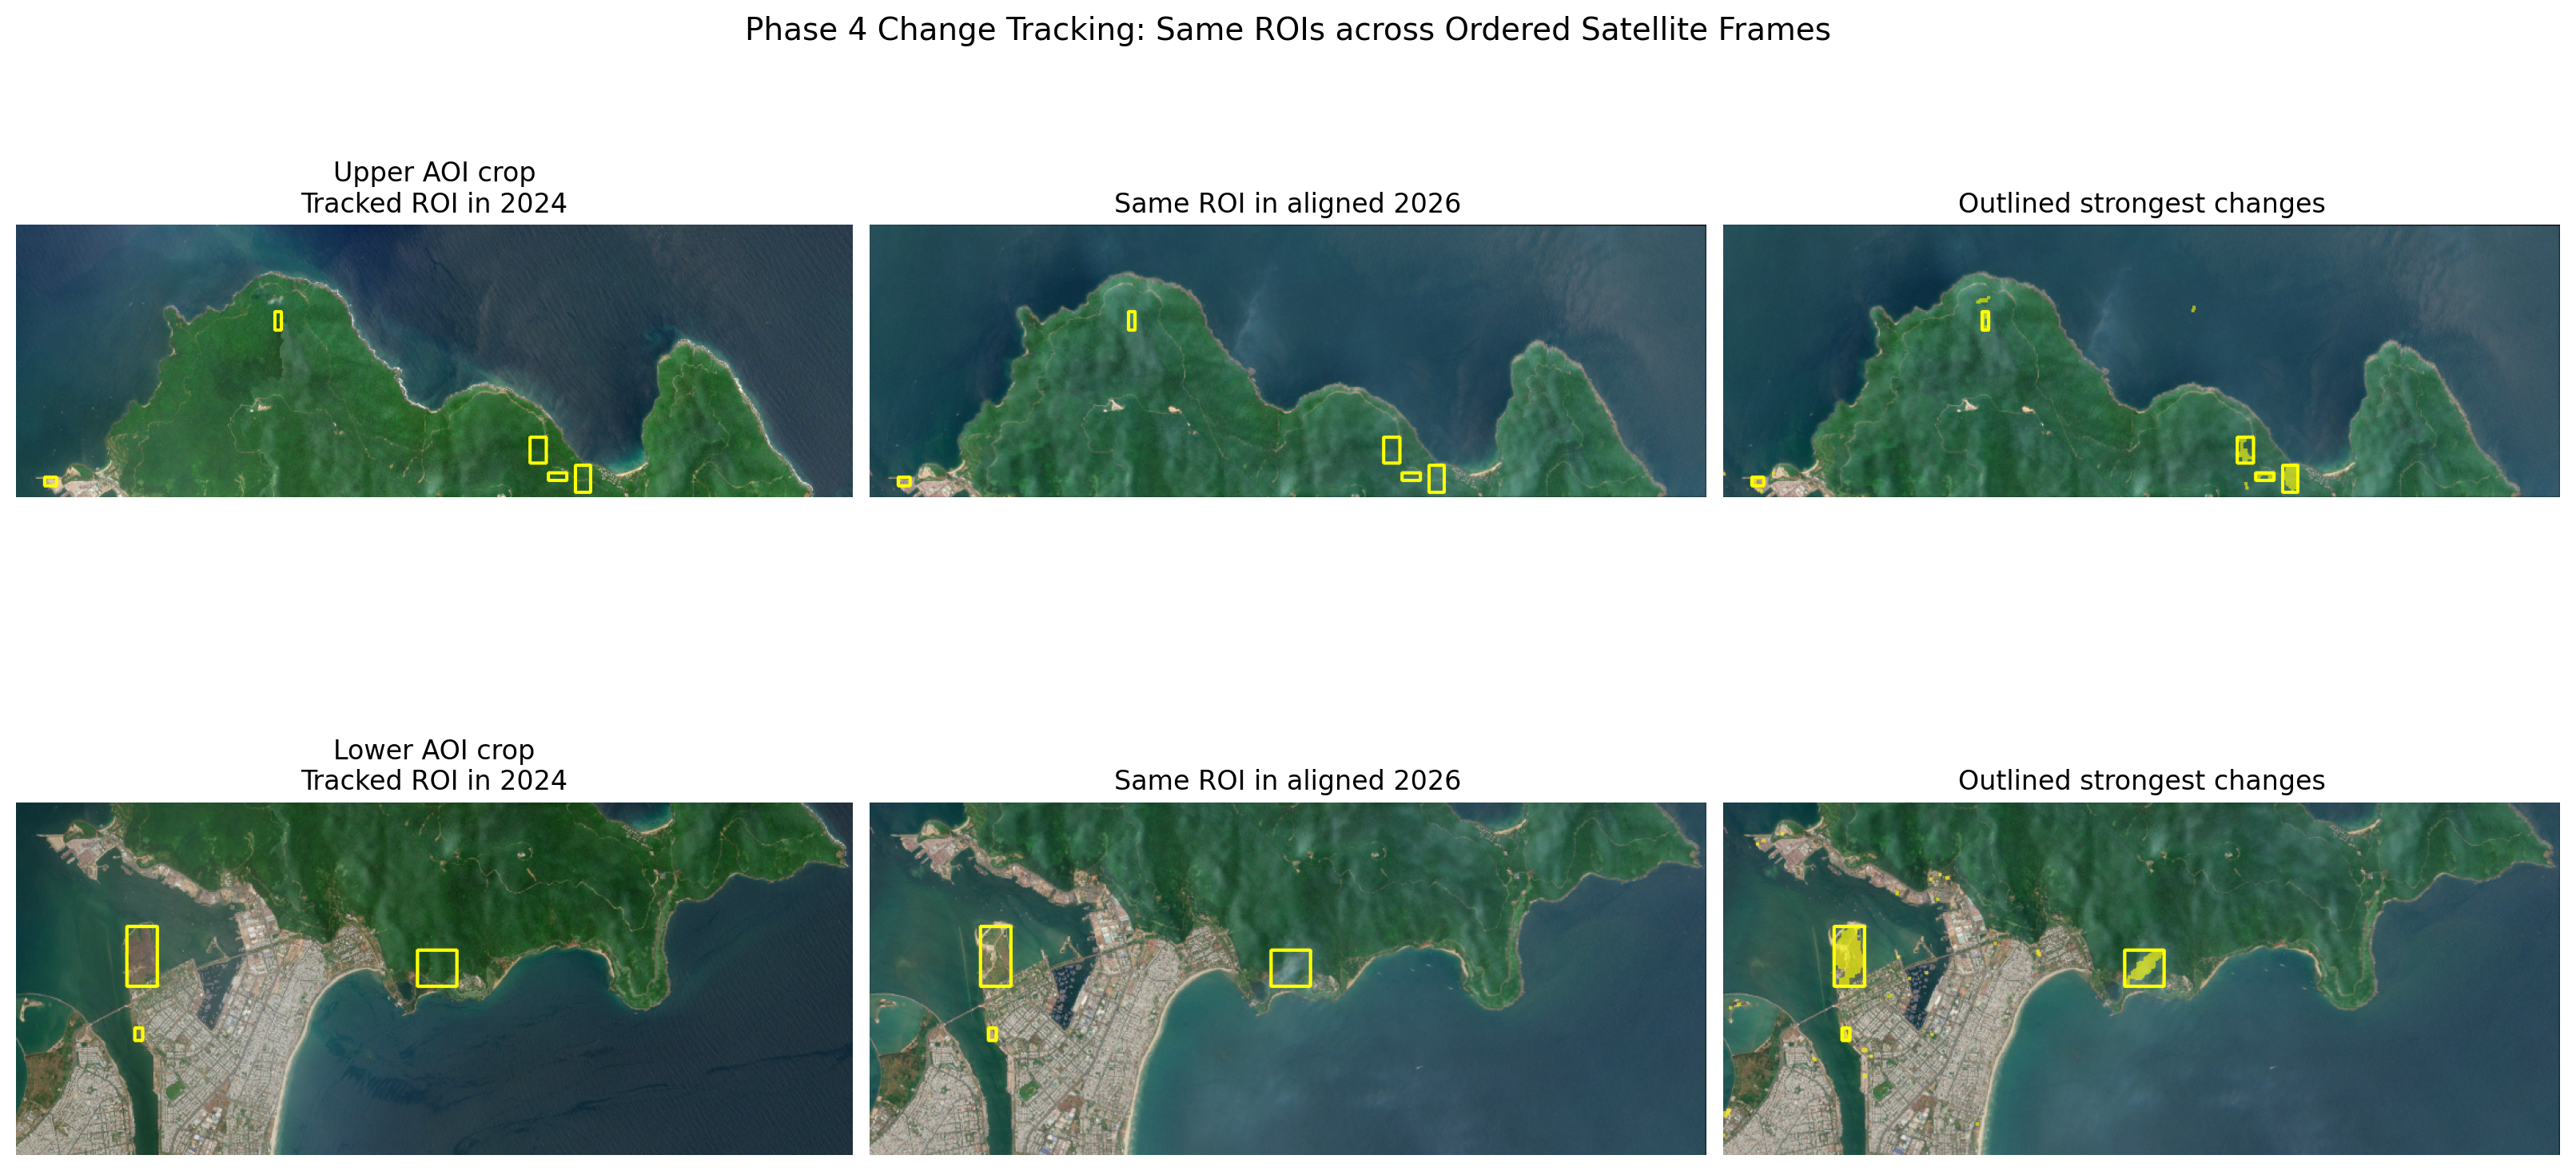
\includegraphics[width=0.98\textwidth]{../output/phase4_top_change_regions_tracking.png}
    \caption{Zoomed-in tracking of the top regions with the most significant urban expansion.}
    \label{fig:phase4_top_change_regions}
\end{figure}

\subsection{False Change Controls}
A major challenge in satellite-based change tracking is the high rate of false positives. To ensure the robustness of our tracking pipeline, we implemented several explicit controls:
\begin{itemize}
    \item \textbf{Misregistration Artifacts:} As demonstrated in Phase 3, slight orbital offsets between satellite passes cause severe edge ghosting. Co-registering the 2026 imagery onto the 2024 frame via SIFT and RANSAC successfully mitigated this geometric source of false change.
    \item \textbf{Clouds and Shadows:} Transient atmospheric effects like clouds and cloud shadows drastically alter pixel reflectance. We explicitly added cloud and shadow rejection filters into our land-cover classifier (using HSV saturation/value and NDVI thresholds) to prevent them from being falsely tracked as "changed" land.
    \item \textbf{Morphological Filtering:} We enforced a minimum contiguous area threshold (e.g., 120 pixels) when drawing bounding boxes. This prevents tiny, isolated noise pixels from triggering the change tracker.
\end{itemize}

\begin{figure}[H]
    \centering
    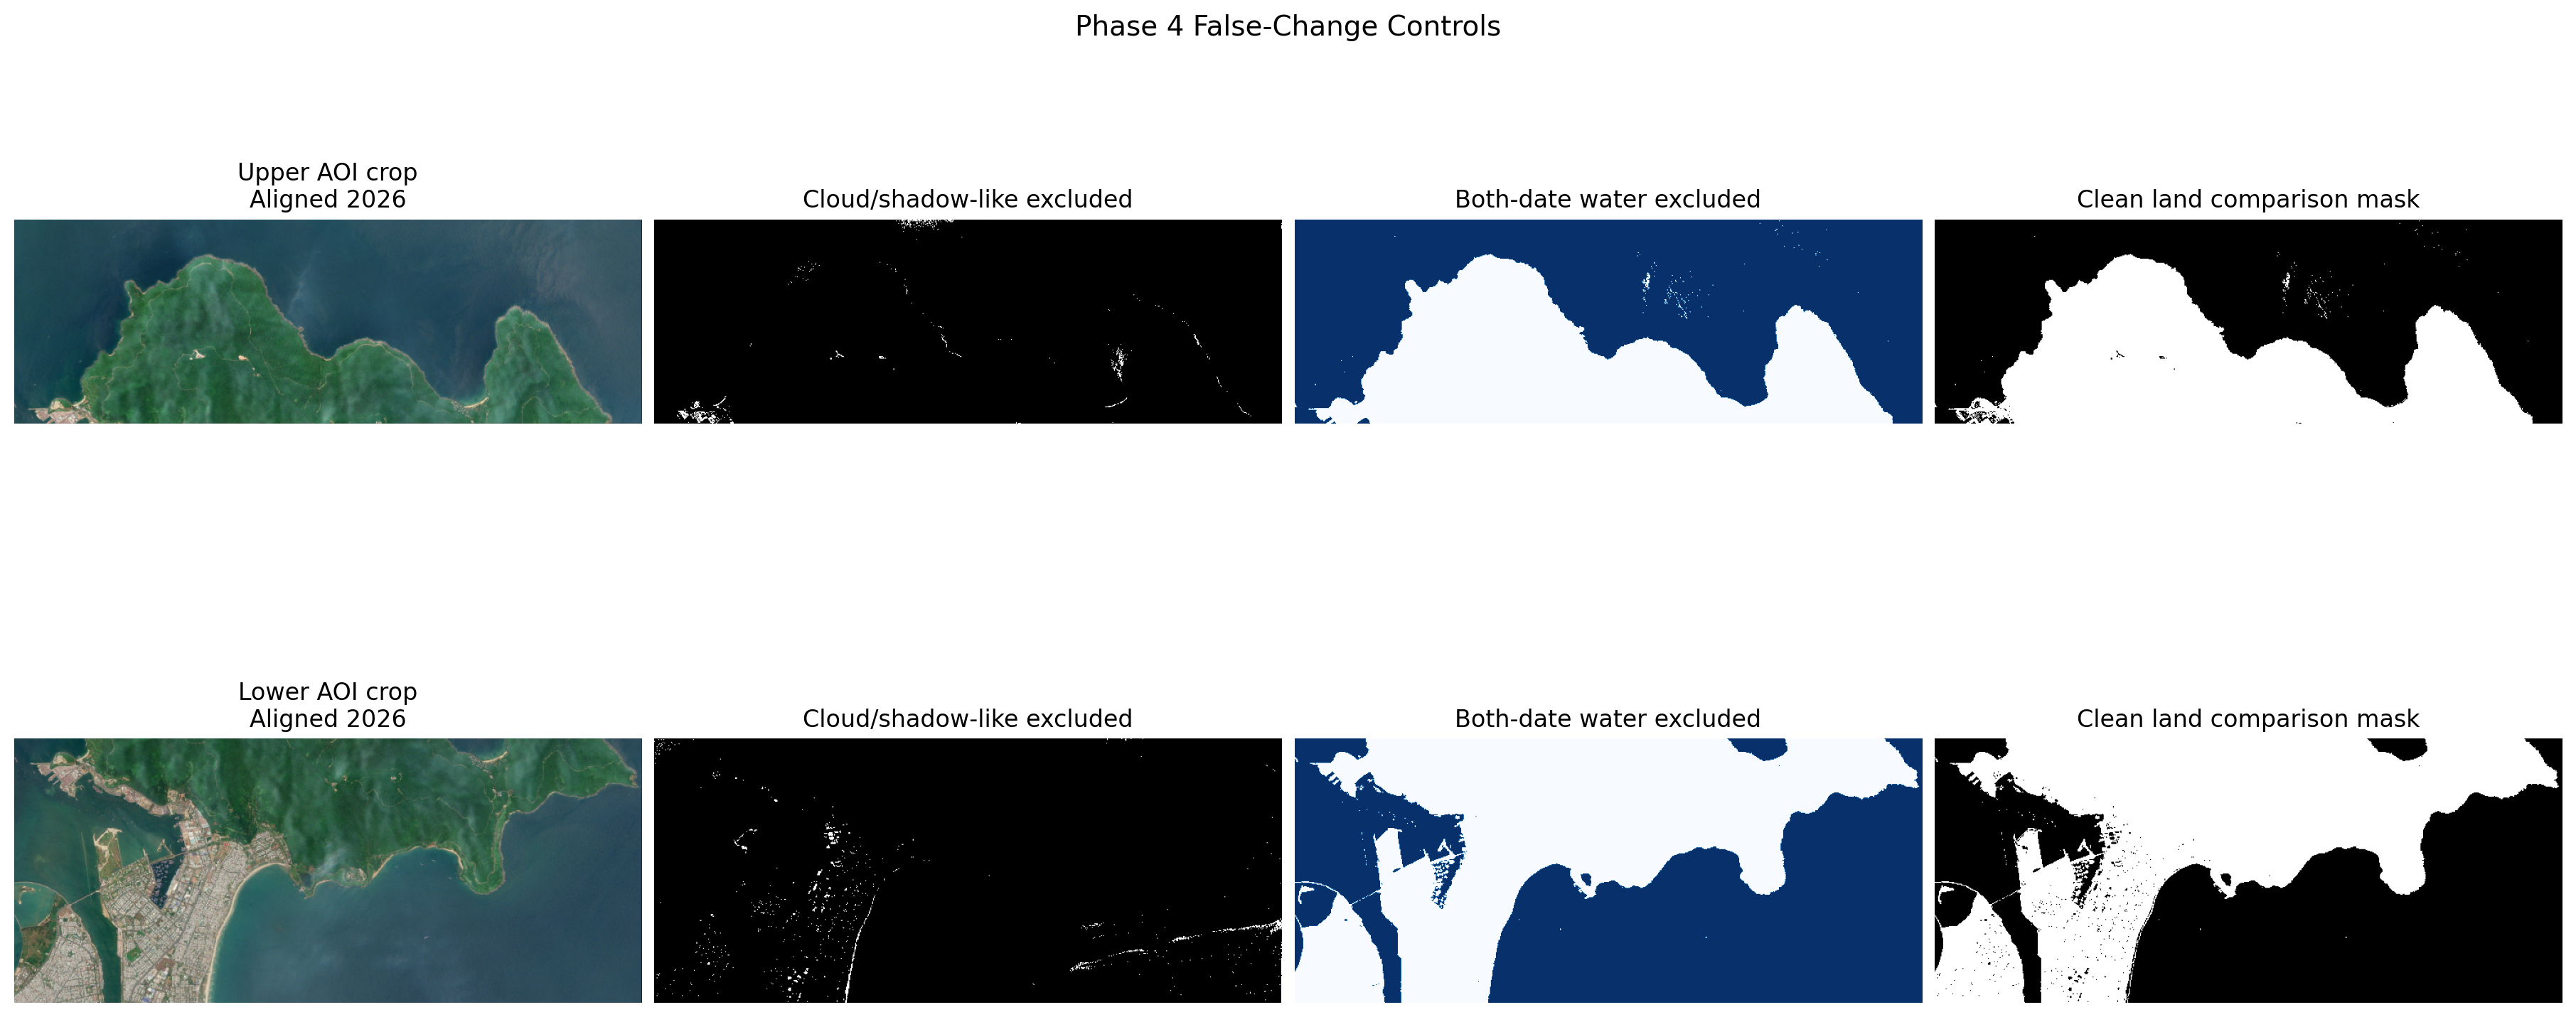
\includegraphics[width=0.98\textwidth]{../output/phase4_false_change_controls.png}
    \caption{Demonstration of false change controls. The pipeline actively rejects clouds, shadows, and isolated noise pixels to ensure only genuine land-cover changes are tracked.}
    \label{fig:phase4_false_change_controls}
\end{figure}

\section{Phase 5: Conclusion \& Reflection}
In this project, we successfully built an end-to-end computer vision pipeline to analyze satellite imagery from Sentinel-2 over Da Nang. By processing multispectral bands, performing feature-based image stitching and temporal co-registration, and ultimately deploying a multi-condition classifier, we detected and tracked urban expansion between 2024 and 2026. 

\subsection{Limitations and Critical Reflection}
Despite the success of our change tracking pipeline, several inherent limitations in satellite remote sensing must be acknowledged:
\begin{itemize}
    \item \textbf{Spatial Resolution Limits:} With a maximum resolution of $10\text{ m/pixel}$ (Bands 4 and 8), fine-grained urban features like narrow residential streets or individual small houses cannot be perfectly resolved. They often suffer from the "mixed pixel" effect, where a single pixel contains spectral signatures of both concrete and surrounding vegetation, leading to classification ambiguity.
    \item \textbf{Atmospheric and Seasonal Effects:} Even though we selected images from the same season to minimize variations, differences in atmospheric scattering (haze), sun elevation angles, and water turbidity between the two passes still introduced slight reflectance variations.
    \item \textbf{Geometric Distortion:} While our SIFT + RANSAC co-registration significantly improved alignment, the push-broom sensor dynamics of Sentinel-2 combined with differing off-nadir viewing angles mean that tall structures (like high-rise buildings) may exhibit parallax displacement (leaning) that 2D homography cannot perfectly correct.
\end{itemize}

\subsection{AI Audit Log}
To comply with the assignment requirements, we utilized various AI assistants (ChatGPT, Claude, GitHub Copilot) to accelerate coding, debug errors, and brainstorm methodological approaches. A comprehensive and detailed log of our AI interactions across all five phases has been submitted separately in the \texttt{ai\_audit\_log\_g3.md} file.

\subsection{Peer Evaluation Form}
The table below summarizes the self and peer evaluations for all members of Group 3. Given the successful completion of all required tasks across the five phases, the team agreed on an equal distribution of effort.

\begin{table}[H]
    \centering
    \caption{Group 3 Peer Evaluation Form}
    \label{tab:peer_evaluation}
    \begin{tabular}{|l|l|c|}
        \hline
        \textbf{Member} & \textbf{Assigned Role} & \textbf{Contribution} \\
        \hline
        DinhHoang & Phase 0: Setup \& Data Collection & 100\% \\
        KhoiNguyen & Phase 1: Image Processing & 100\% \\
        ThaoHien & Phase 2: Segmentation \& Features & 100\% \\
        NhaTran & Phase 3: Alignment \& Stitching & 100\% \\
        GiaBao & Phase 4: Detection \& Change Tracking & 100\% \\
        AnhKiet & Phase 5: Reporting \& AI Audit Log & 100\% \\
        \hline
    \end{tabular}
\end{table}

\textbf{Peer Evaluation Comments:}
\begin{itemize}
    \item \textbf{DinhHoang:} Excellent data curation and preprocessing.
    \item \textbf{KhoiNguyen:} Solid implementation of NDVI and filtering.
    \item \textbf{ThaoHien:} Great work on Mean-Shift and validation.
    \item \textbf{NhaTran:} Handled complex SIFT/RANSAC logic well.
    \item \textbf{GiaBao:} Built a robust tracking and filtering pipeline.
    \item \textbf{AnhKiet:} Consolidated report and structured the logs.
\end{itemize}

\end{document}
